\chapter{Screen-based semantic speech editing}

\section{Introduction}
Speech is a natural form of communication which is rich in information. Since
the early twentieth century, radio broadcasting has been used to transmit and
consume speech-based content. Today, radio listenership remains high and
podcasting continues to grow in popularity. 

Although many radio programmes are still broadcast live, a large proportion are
pre-recorded and put together using audio editing software. Efficient
navigation and editing of speech is crucial to the radio production process.
However, unlike text, speech must be consumed sequentially, and does not
naturally support visual search techniques \citep{Wolfe2004}. 

Audio editing interfaces display a visual representation of the amplitude of
the sound, called a `waveform'. This gives users some ability to visually
search and scan audio content. Although the waveform is useful for many editing
tasks, it displays very limited information, especially when zoomed out
\citep{Loviscach2011}.

Semantic audio analysis technology can be used to extract higher-level
information from the sound, such as whether it is speech or music
\citep{Panagiotakis2005}, where different people are speaking
\citep{AngueraMiro2012} or an approximate transcript of what they are saying.
Presenting this information to the user could allow them to navigate and edit
audio content much more efficiently \citep{Whittaker2004}.

In this paper, we investigate semantic speech editing in the context of
professional radio production. We explore what the typical production process
is, including the workflow and tools that are used. Based on our
analysis, we then introduce a semantic audio editing system that automatically
transcribes speech recordings, and allows users to navigate and edit the speech
using the text of the transcript.  We evaluate the resulting system though a
qualitative study of professional BBC radio producers who use our semantic
editor to create real radio programmes for broadcast.

% RESEARCH QUESTIONS?

\section{Related work}\label{sec:relatedwork}
%For example, it can be
%used to distinguish between music and speech \citep{Wieser2014}, show where
%different people are speaking \citep{AngueraMiro2012}, and who those people are
%\citep{Doddington1985}. These technologies have successfully been combined to
%create an enhanced interface to large speech archives as part of the BBC World
%Service Radio Archive
%prototype\footnote{\url{http://worldservice.prototyping.bbc.co.uk/}}.

%Other methods of improving speech navigation have been explored, including time
%compression \citep{Arons1997} to increase playback speed, and using dichotic
%presentation \citep{Ranjan2006} to play different parts of the speech into each
%ear.

Semantic speech editing techniques have been used to enhance a number of
interfaces in a variety of applications by using either manual or
automatic transcription.
%Automatic speech recognition technology makes it possible to extract partially
%accurate transcripts of speech recordings.
%A number of researchers have
%experimented with using these transcripts to enhance interfaces for interacting
%with audio content.
%\subsection{Navigation}
SCAN \citep{Whittaker1999} is an interface designed to support retrieval from
speech archives. It used automatically generated transcripts to allow users to
search for keywords, and to visually search the recording by reading the
transcript. This system was developed into SCANMail \citep{Whittaker2002}, an
interface designed for interacting with voicemail. It added a number of
features including paragraph segmentation and the ability to skip to a point in
the transcript by clicking on a word. The interface was later enhanced with
error correction functionality and confidence shading, which greys-out words
that may be incorrect \citep{Burke2006}. An evaluation of SCANMail using eight
expert users found that the transcript display enabled users to visually scan
the content of recordings to quickly extract information and judge which
parts were relevant, without having to play the audio.

Avid released a feature for their Media Composer video editing software in 2007
called `ScriptSync' \citep{Avid2011}. This feature aligns a user-supplied
transcript to a video recording. The feature places a marker in the video for
each line of the transcript, allowing users to jump to a particular line, or
see which line in the transcript corresponds to the current point in the video.
We did not find any user studies of ScriptSync reported, and the feature was
discontinued in 2014 due to a licensing issue.

Transcripts can also be used as a mechanism for editing media content.
\mbox{SILVER} \citep{Casares2002, Long2003} is a video editor that included
various `smart editing' features including an editable transcript window. It
used speech-to-text to align the words from subtitles to video. The video could
then be edited by selecting and deleting text in the transcript. Gaps, errors
and edits were displayed in the transcript using special characters and the
user could correct missing or wrong words. All of the video editor's features
were evaluated together in an informal study with seven students. The report of
the study did not provide any results on the transcript-based editing
feature.

When editing a video interview, you want to avoid making a cut when the person
speaking is in shot, because it causes the image to suddenly jump.
\citet{Berthouzoz2012} used image processing algorithms to create a video
editor that can help the user hide these edit points. The editor has an
editable transcript window that displays suitable edit points and allows the
user to edit the video by selecting and deleting text. The transcripts were
generated using a paid-for crowd-sourcing service with speech alignment
software. The system also allowed users to easily remove `umm's or repeated
words. No user study was conducted in the reported study, however positive
feedback was received from nine professionals who were given a demonstration.

\citet{Whittaker2004} created an interface for editing
voicemail messages using automatically-generated transcripts. Users could
cut-and-paste parts that they wanted and delete other parts.
The system was evaluated in a formal study of 16 voicemail users, which found
that semantic editing was faster and as accurate as editing with a
waveform-based interface. Crucially, this was true even though the transcripts
had an average word error rate of 28\%. This shows that semantic editing is
beneficial even when using imperfect transcripts.

Hyperaudio Pad is an open-source audio and video editor, first proposed by
\citet{Boas2011}, and now available online as a free service
\citep{Hyperaudio2016}. This is a web-based interface that allows users to
navigate and edit online media using transcripts. The transcripts are generated
from subtitles by using speech alignment software. Editing is done by selecting
a part of the transcript and dragging it into a window to create a `clip'.
Other clips can be added and re-ordered, and the edited version can be played
and shared with others. No user studies of this system could be found.

\citet{Rubin2013} presented a novel interface for creating `audio
stories' that combine speech and music. The interface uses an editable
transcript with two columns, one for each of a pair of speakers.  It allowed
the user to cut, copy, paste and delete the audio using the text. It also
highlighted repeated words, similar sentences, `umm's, breaths and pauses in
the transcript. The transcripts were generated using a crowd-sourcing service
with speech alignment software that also detected breaths.  The system from
Rubin et al. included additional functionality for finding and adding music
tracks, and for varying the length of music using automatic looping. The system
was evaluated through a short informal study of four participants where the
editing capabilities received positive feedback. No follow-up studies have been
reported since.

Recently, \citet{Sivaraman2016} created a semantic editing system for
asynchronous voice-based discussions, where users could quickly edit their
speech recording before sending it to the recipient.  Their system used
near-live automatic transcription and detected pauses in the speech. Their
interface allowed users to delete selected words/pauses, insert
additional pauses and fix incorrect words.  In a formal study of their system
with nine users, they found that text-based editing was considered good enough
to replace waveform editing, and to be more accessible. They observed that most
users only used the system to make fine-grained edits, instead of editing large
chunks.  Users said that the transcript also allowed them to quickly
review all the points that were made, and that the errors in the transcript
weren't a heavy distraction.

%\subsection{Time compression}
%A number of studies \citep{Whittaker2002,Vemuri2004,Ranjan2006} have also
%combined transcript displays with time-compression to speed up playback of
%audio. They found that having a transcript improves comprehension and allows
%faster playback.

%Dichotic presentation, in which different parts of a recording are played into
%each ear, was also tested \citep{Ranjan2006}.

%\begin{figure}
%\centering
  %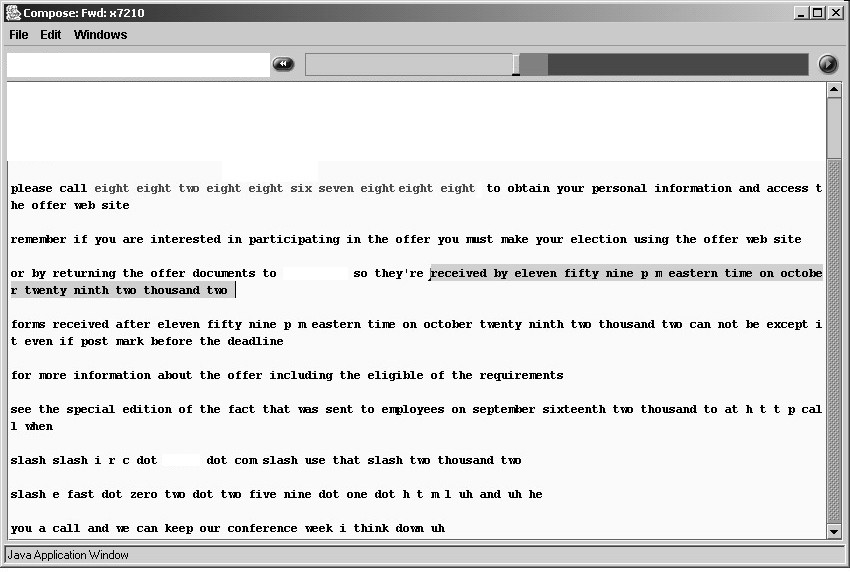
\includegraphics[width=\columnwidth]{figures/whittaker2004.png}
  %\caption{Semantic speech editor \citep{Whittaker2004}}
  %\label{fig:semanticeditor}
%\end{figure}

%, which has been shown to improve the speech and
%accuracy of audio search \citep{Ranjan2006,Whittaker2000} and comprehension
%\citep{Vemuri2004}. Word-level timing information, also allow users to edit
%speech using a text-based interface \citep{Whittaker2002,Burke2006,Rubin2013}.
%Even with imperfect transcriptions, editing using this technique is faster and
%as accurate as acoustic editing \citep{Whittaker2004}.

%Later systems have improved these interfaces with editing \citep{Burke2006},
%confidence shading \citep{Burke2006} and highlighting breaths, pauses and
%repetition \citep{Rubin2013}.

In summary, \citet{Whittaker2004} found that semantic editing of speech in
voicemail is faster and as accurate as using waveforms.  \citet{Sivaraman2016}
found that for editing discussions, semantic editing is a more accessible
alternative to waveform editing. Systems have been developed for audio and
video production \citep{Casares2002,Berthouzoz2012,Rubin2013}, but these were
mostly designed without prior user requirements, and the studies were informal
and used amateur participants. In this paper, we describe the design of our
system, which is based on the results of a published pilot study, and present
our formal study, which uses real content and professional users in an
uncontrolled working environment.

%, however most of these were
%developed without prior user requirements, none of them were tested in a formal
%user study and the informal studies that were conducted used amateur
%participants. Additionally, these In this paper we introduce Dialogger, a semantic speech editing
%system whose design is based on real-world requirements, and present the
%results of a formal user study of the system in an uncontrolled professional
%working environment.

%These studies have demonstrated the potential that transcript-based interfaces
%have for improving the navigation and editing of audio content. However, they
%have not yet been tested under real-world conditions.



%In this section, we review
%the results of the study and how it shaped the design of our system, before
%describing the features and the interface.



%We created our prototype semantic editing system `Dialogger' to assist
%specifically with the logging and rough editing stages of radio production.
%Dialogger allows users to upload audio recordings which are then transcribed
%and presented in a text-based interface that allows them to navigate and edit
%the audio using the transcript.  Dialogger then allows them to export their
%edit directly into a digital audio workstation (DAW) without loss of quality,
%where they can continue with their normal production workflow.

%In order to determine how these technologies would be best applied in the
%context of radio production, we conducted a short pilot study of radio
%production at the BBC, the results of which are more fully documented in
%\citep{Baume2015}.

%, which explored the workflow, roles, motivations and
%environmental factors.

\section{System requirements}\label{sec:requirements}
Our interest in applying semantic editing techniques to radio production first
emerged from a pilot study we conducted at the BBC \citep{Baume2015}.  In this
section, we discuss the findings of the study and the resulting system
requirements for our semantic editing system.

\subsection{Pilot study}
The objectives of the pilot study were to discover how
radio programmes are created, and to identify any opportunities to improve the
process.  Three representative programme types were studied: a
news bulletin, a drama and a documentary. The producers of each programme were
observed and interviewed to fully document their workflow, which took between
half a day (for news) and four days (for the documentary).

The main finding of the study was that many producers prefer to work with
text-based representations of audio, rather than working with the audio
directly. For example, the producers of the documentary `logged' each interview
they recorded by transcribing it themselves, or by
paying a third-party service to write a full transcription.  They then used the
transcripts to select which bits they wanted to use, and copied the text to
create a rough script of the programme. Once the script was mostly complete,
they had to find and cut each piece of audio for the programme to create what
is known as a `rough edit'.  Both the logging and rough edit processes are very
time-consuming for the producer.  From this study, we identified an opportunity
to apply semantic speech editing techniques to these parts of the production
workflow.

\subsection{Transcripts}
Radio programmes are assigned a slot in the broadcast schedule, so producers
have a strict deadline for finishing their programme. Programmes are often
scheduled about three weeks in advance, but sometimes as little as a week in
advance. This means that producers have very little time to spare. If a
programme's budget allows, interview recordings can be sent to a transcription
service where they are transcribed by a person within about 24 hours. However,
most programmes do not have the budget for this, so the producer transcribes
the recordings themselves.

Transcripts are used to help the producer make editorial decisions, but are
usually not published. For this reason, the transcripts only have to be
sufficiently accurate to use for editing. Both \citet{Whittaker2004} and
\citet{Sivaraman2016} found that the errors in the transcripts did not prevent users
from being able to edit using them. However, both also found that
users wanted to be able to fix incorrect words in the transcript.

Our semantic editing system needs to be able to produce a transcript quickly
and cheaply. It should be accurate enough to be useful for editing, and allow
for correction where necessary.

\subsection{Editing}
There are already well-established systems and software in place for producing
radio programmes. Producers use a digital audio workstation (`DAW') to select
the parts of each interview that they want to use in their programme, and to
arrange them into a narrative. The BBC provide two different DAWs -- dira!
StarTrack (made by SCISYS) and SADiE (made by Prism Sound). Some producers
prefer to use other DAWs, but as installation of software is restricted on
corporate computers, they must use their personal computers.

Waveforms are used to visually represent audio in the DAW to help the user
navigate the recordings. The edits performed in a DAW are `non-destructive'
because the original recordings remain untouched. This allows the producer the
flexibility to adjust or undo their decisions at any point during the editing
process.

Specialist sound engineers (known as `studio managers') are sometimes brought
in on the last day of production to ensure that the sound is well balanced, and
to do any advanced editing that is required. This includes removal of
unwanted `umm's or breaths in a process called `de-umming'. Being able to
de-umm speech in a way that is inaudible to the listener is a skilled task that
requires precision and experience.

Music is often included in a programme, either as a theme tune, a short
interlude or in the background. Producers select the music, often from their
personal collection. However, a number of services are also used for finding
suitable commercial or rights-free music, such as Audio
Network\footnote{\url{https://www.audionetwork.com/} (accessed 15.08.2016)}.
The music is added and edited using the DAW.

At the end of the editing process, the producer's supervisor (known as the
`editor') listens to the programme with the producer to give their feedback and
sign-off. As part of this process, they both listen out for repeated words or
phrases. However, this is only usually a problem in drama production where
multiple takes of the same lines are recorded.

Our semantic editing system needs to be able to select and arrange parts of
audio recordings. Given that there are established radio production
systems for advanced tasks such as de-umming and addition of music, it also
needs to be able to integrate with these so that it can be used in 
professional radio production.

% - Select parts of recordings and arrange into order
% - 

% Transcription
% X Need transcripts quickly
% X Not much money for transcripts
% X Transcripts aren't published, need to be good enough (Whittaker2004)
% X Whittaker says that correction would be good
%
% Integration
% X Existing system in place for broadcasting
% X Currently use waveforms
% X Must be non-descructive
%
% Web-based
% X New software can't be installed
%
% Drag and drop
% X Production involves picking bits out of interviews
% X Sorting, trying out different orders
%
% Umms/breaths
% X De-umming is skilled and done in DAW
%
% Music editing
% X Music discovery is done using existing systems
% X Editing is done in DAW
%
% Repeats
% X Repeats don't happen in interviews, only in drama really

\section{System design}
This section describes our system design, as guided by the requirements set out
in Section~\ref{sec:requirements}, followed by a description of the system.

\subsection{Transcript}
Three factors were considered when choosing a transcription method --
turnaround time, cost and accuracy. Manual transcriptions are nearly 100\%
accurate, however they are expensive (about \$1 per minute) and slow (typically
24 hours). Automatic transcriptions are imperfect, but cheap (about \$1 per
hour) and fast (x2 real-time). Our system requires quick and cheap transcripts
that are sufficiently accurate, so we chose to use automatic transcripts
generated by a state-of-the-art commercial web
service\footnote{\url{https://www.speechmatics.com/} (accessed 15.08.2016)}.

Automatic transcriptions were also used by \citet{Whittaker2004} and
\citet{Sivaraman2016}, but \citet{Berthouzoz2012} and \citet{Rubin2013} chose
to use perfect transcripts from a crowd-sourcing service. \citet{Hyperaudio2016}
used aligned subtitles and \citet{Casares2002} used a combination of subtitles
and speech-to-text.

\subsubsection{Accuracy}\label{sec:transcript}
In an informal evaluation of our speech-to-text system which used 48 hours of
mixed-genre television content, it had an overall word error rate of 47\%.
However for news content, which is clearly spoken by a native speaker, this
dropped to 16\%. As the speech on radio programmes is similar in nature to
speech on television news, the error rate was comparable. However recordings
with non-native speakers or significant background noise had a higher error
rate. For comparison, the reported error rate of the system used by
\citet{Whittaker2004} was 28\%, and for \citet{Sivaraman2016} it was 10\%.

\citet{Whittaker2004} and \citet{Sivaraman2016} found that users want to be
able to correct the transcript. We designed the system so that users can change
words by double-clicking them, typing the correct word and pressing enter.
\citet{Casares2002} also provided correction functionality, but the other
systems did not include this feature as they used perfect transcripts.

\subsubsection{Speed}
The time taken by the transcription service to process each uploaded recording
was approximately half as long as the length of the recording. The time
depends primarily on the length of the recording but also on noise, accents and
the complexity of the speech.

\subsubsection{Additional information}
The speech-to-text system we chose to produce transcripts generates
additional information from the audio. It attempts to identify the people
speaking in the recording by their gender and a number (e.g. [M2], [F5]). Also,
for each word, the system assigns a value between 0 and 1 of how confident it
is that the word is correct. We decided to include these extra pieces of
information, as they should both be useful to the producer.

We labelled each paragraph in the transcript to indicate where different people
are speaking. \citet{Rubin2013} also identified speakers by placing their
respective parts of the transcript in different columns.  However, this
approach limits the number of speakers by the number of columns that can be
displayed. By labelling paragraphs, we are able to support multiple speakers.

We used the confidence value for each word to shade words that fell below a
threshold, using a technique known as `confidence shading'. This has previously
been used by \citet{Burke2006} for navigation of speech, but it has not yet
been used for semantic editing.


%The speech-to-text system can recognise esoteric words like `ribosome' and
%`ARPANET', but can struggle with colloquialisms and casual conversation. If the
%recording is too quiet or noisy, or a word isn't in its dictionary, the system
%makes a best guess (e.g. `subbuteo' was translated as `some beauty'). It also

%Recorded interviews have at least two people speaking (sometimes more), so it
%is helpful to know where in the recording they are speaking. Our system
%attempts to detect where there is a change of speaker, then inserts a new 
%paragraph for each speaker with a unique label including their gender (e.g. M2, F5).
%We selected this layout over Rubin's approach of having separate columns
%for each speaker so as to allow more than two speakers.

\subsection{Interface}
Our semantic editing system needs to be able to select and arrange parts of
audio recordings. To achieve this, we used the same drag-and-drop interface as
\citet{Hyperaudio2016} as it is a simple method for extracting and re-ordering
clips. It also allows clips from different recordings to be added and
re-arranged. \citet{Casares2002}, \citet{Sivaraman2016} and
\citet{Berthouzoz2012} used a select/delete interface, where parts of an
individual transcript can be chosen or removed, and \cite{Whittaker2004} and
\citet{Rubin2013} used a cut/paste/delete interface.

We designed our interface to be browser-based, as the BBC corporate policy
meant that it was not possible to install new software on the producers'
computers. This came with the added benefit of allowing users to work from
anywhere in the world on any operating system, but the downside that they have
to be connected to the Internet.

\subsection{DAW integration}
Our system needs to be able to integrate with the existing radio production
tools. We designed Dialogger to be used as the first stage of the editing
process, and to smoothly integrate with the DAWs that are used in BBC Radio. We
achieved this by providing a novel features to export edited content from our
system, either as a .wav audio file or as an `edit decision list' (EDL).

The first option exported a single .wav audio file of the edit. This method is
a `destructive' edit, in that it throws away the pieces of the recording which
weren't selected. 
The other option exported an EDL, which contains metadata about which parts of
an audio or video recording make up an edit. These can be read by the
two most common audio editors used at the BBC -- SADiE and dira! StarTrack.
This method is `non-destructive' because the full original recordings are
retained and the edit points can be re-adjusted in the audio editor.  Following
early informal feedback, features were added to allow the text to be printed or
exported into a word processor.

\subsection{Excluded features}
\citet{Rubin2013} and \citet{Berthouzoz2012} included detection and removal of
`umm's or breaths as this was generated as part of the crowd-sourcing service.
We did not include this functionality as we found during the pilot study that
removal of `umm's and breaths is a highly specialised task that cannot yet be
automated to a professional standard.  Additionally, as our system is based on
speech-to-text, information about the position of `umm's and breaths is not
available.

We did not include features for adding or editing music. During the pilot study,
we found that specialist tools are already used for finding and choosing music,
and that editing of music is already efficiently handled by the DAW.
\citet{Rubin2013} included features for finding music tracks and creating loops
within them.

\citet{Rubin2013} also included detection of repeated words and phrases. We
chose not to include this, as our pilot study found that repeats are only an
issue in drama production. As the production of drama involves a very different
workflow \citep{Baume2015}, we chose not to include drama production in our
system design or study.

%\begin{figure}
%\centering
  %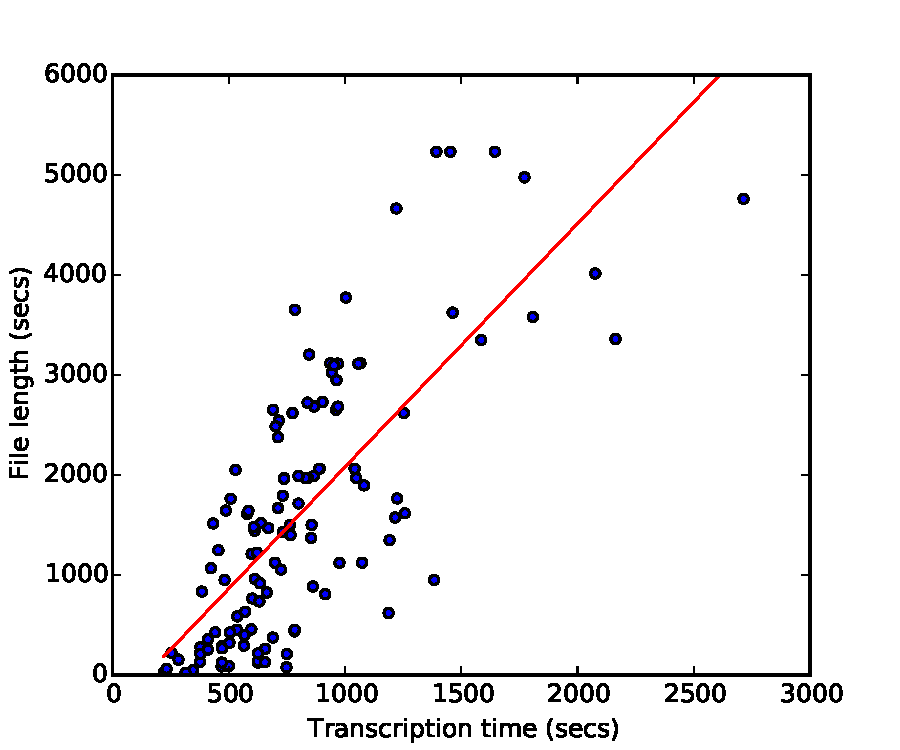
\includegraphics[width=\columnwidth]{figures/transcribetime.pdf}
  %\caption{Time taken to transcribe each recording with linear trend line}
  %\label{fig:transcribetime}
%\end{figure}

\subsection{System description}
This section gives a brief overview of Dialogger, including its functionality
and operation.  A screenshot of the interface and numbered list of the main
features are shown in Figure~\ref{fig:interface}.  A live demo of the system
is also available\footnote{\url{https://speecheditor.virt.ch.bbc.co.uk/demo}
  (accessed 15.08.2016)}.

\begin{figure*}[ht]
\centering
  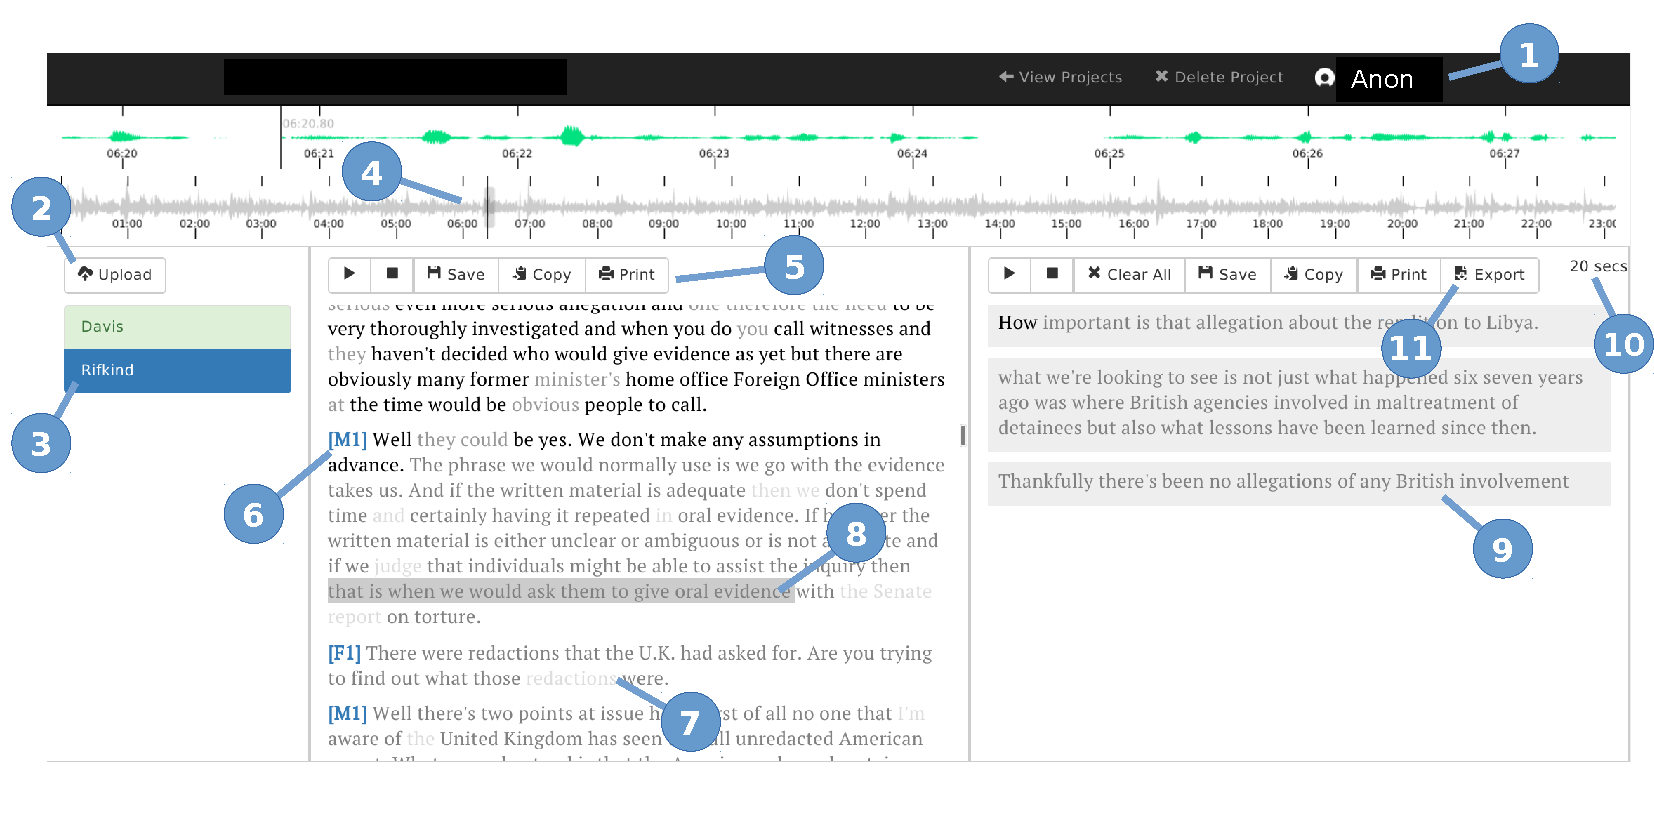
\includegraphics[width=\columnwidth]{figs/interface-labels.pdf}
  \caption{Screenshot of the user interface with highlighted features: (1)
    individual user accounts and projects, (2) upload of audio recordings, (3)
    list of uploaded recordings, (4) waveform display of currently selected
    recording, (5) toolbar with playback, save, copy and print functionality,
    (6) transcript of selected recording with speaker labelling and word
    editing, (7) confidence shading, (8) transcript selection with
    drag-and-drop editing, (9) listing and re-ordering of edits, (10) duration
    of edit, (11) export edit to audio file or digital audio workstation.}
  \label{fig:interface}
\end{figure*}

\subsubsection{Functionality}
Dialogger is web-based speech editing tool that can be accessed from anywhere
using a web browser.
Users can upload their own speech recordings into a project in their individual user
account. Each recording is automatically transcribed at around twice
real-time speed, with a word error rate of approximately 16\%.

The interface displays a list of the user's recordings on the left, the
transcript of the selected recording in the middle, and a blank workspace on the
right. The waveform of the selected recording is also shown at the top.
Users can play a recording, and navigate it using either the transcript or the waveform.

The transcript is divided into paragraphs at points where the speaker
changes. Each paragraph is labelled with the speaker's assigned identity, including
their gender (e.g. [M3]). Words that might not be correct are shaded grey, and
incorrect words can be fixed by the user. Buttons at the top of the transcript
allow the user to print the transcript, or copy it into a word processor.

Recordings can be edited by highlighting and dragging words from the
transcript to the workspace on the right, which creates a clip. Multiple clips
can be created and re-ordered to produce an edited version. The edited version
can be played to allows users to preview the result. The user can save their
edit to revisit later.

The interface displays the total duration of the edit. The edited version can
be exported as either a .wav audio file, or as an edit decision list (EDL) for
a digital audio workstation (DAW).

%TODO Add block diagram?
\subsubsection{Operation}
The operation of the system is described below as a typical user journey. Each
feature is numbered and shown in Figure~\ref{fig:interface}.

Users access Dialogger by navigating to a web page in their browser. They start
by logging into the system using their account (1) and create a project where
they can upload their speech recordings (2) that appear in a list on the left
(3). Each recording is automatically transcribed. When it is opened, the
waveform appears at the top and the transcript appears in the middle section.
The recording can be played (5) and navigated by using the waveform (4) or by
clicking on a word in the transcript (6). The transcript shows where different
people are speaking with labels at the beginning of each paragraph. Words which
are likely to be incorrect are shaded grey (7), known as `confidence shading'.
Incorrect words can be fixed by double-clicking them and typing the correct
word. The audio can be edited by selecting a range of words (8), then using
drag-and-drop to place it in the area to the right which creates a clip (9).
Clips can be re-ordered and deleted. The total duration of the edited clips is
displayed (10). The edited clips can be exported as a .wav audio file or as an
EDL (11) for further editing in a DAW.

%During this period there was no easy
%way to listen to the audio, so although they know \textit{what} was said, they
%don't know \textit{how} it was said.

%After editing using the transcript, the producer must go back to find and cut
%each piece of audio they wanted to use in the programme, known as a `rough
%edit'. Moving from audio to text and back again is costly, but is considered
%by the producers to be worthwhile. We believe that by linking audio and text
%representations together in a single editing system, it would be possible to
%work with either representation without incurring the cost of converting
%between the two.

%The pilot study also found that some of the functionality included in previous
%studies is already efficiently handled, or cannot yet be automated. For
%example, advanced music discovery platforms like Audio
%Network\footnote{\url{https://www.audionetwork.com/}} allow producers to
%quickly find music tracks of the right length, and removing `umm's or breaths
%from speech transparently is a skilled task that requires fine editing and
%human judgment.

 %It found that producers of speech radio prefer to work with
%text-based representations of audio rather than with the recordings directly.
%Their workflows are primarily paper-based which creates extra work when moving
%between paper and audio. Creating a link between the words on the paper and
%their location in the audio recordings could significantly improve the
%production workflow.

%The study also identified opportunities to apply semantic audio technology
%and interaction design to radio production tasks. Lots of time is spent
%cleaning up recordings by removing redundant speech, which could be fully or
%semi-automated. Segmenting speech content by speaker would make a positive
%impact on most speech-based tasks. Finally, drama productions could benefit
%from an easy way to compare multiple takes of the same scenes.

%\subsection{Design}
%We designed Dialoger to play to the strengths of transcript-based editing by
%focusing on the key features for logging and rough editing, and integrating
%well with the current production workflow. We excluded some features like
%removing `umm's or adding music, which are better handled by existing systems
%or techniques.  We also excluded detection and handling of repeated phrases, as 
%this technique is only used in drama production.

%This section describes the design, features and implementation of the
%prototype.




%\subsubsection{Transcription}
%\subsubsection{Layout}
%The interface is laid out so that the workflow operates from left to right.
%Recordings are uploaded and listed on the left (2), the transcript of the
%currently selected recording is shown in the middle (6), and clips are
%created and exported on the right (9). The waveform of the currently selected
%recording is shown at the top on a dual time-line (4), where the bottom
%waveform shows the entire recording and the top is a magnified display of the
%current position.

%\subsubsection{Navigation}
%Users can navigate the selected recording by clicking on a word in the
%transcript, which seeks to that position and starts playback, or by clicking on
%the waveform to jump to a specific time. Playback can also be controlled using
%buttons in the toolbar above the transcript (5).

%The text before and after the current playback position is coloured black and
%dark grey, respectively, to indicate the current playback position in the
%transcript.  Words which the speech recognition system is not confident about
%are shaded in light grey (7), known as `confidence shading'.


%\subsubsection{Editing}
%An audio clip can be created from the transcript using drag-and-drop.  The user
%selects text from the transcript (8) then drags and drops the selection in the
%space to the right.  Each clip is contained in a shaded box (9) which can be
%re-ordered by dragging them up and down, or deleted by clicking an `X' in the
%top right of the box.

%The clips can be played using the playback buttons at the top, or by clicking
%on a word. The total length of the clips is displayed above the text (10).


%\subsection{Implementation}
%The system was implemented using web standards, which allowed a consistent
%experience on any recent web browser, and avoided the need to install any
%software locally. The front-end was written in Javascript using the Hyperaudio
%\citep{Hyperaudio} and peaks.js \citep{Peaks} libraries, and the back-end was
%built using Node.js and MongoDB running on a virtualised Ubuntu server.
%Communication between the two was done through a REST API.

\section{Methods}\label{sec:methods}
We designed and conducted a formal study to explore how radio programmes are
currently created, to evaluate how Dialogger performs in professional radio
production, and to measure its impact on the production workflow. 

\subsection{Design and procedure}
Gaining access to radio producers can be difficult as there are not many of
them and they are normally very busy. A number of unrelated
studies on television production systems have previously been conducted
\citep{Engstroem2010,Perry2009}, but we were unable to find any studies at all
which used radio producers. One study attempted to recruit radio producers but
was unsuccessful because the producers were ``so highly tasked''
\citep{Kim2003}. However, we were able to recruit professional radio producers
from the BBC due to the access available to us as an internal research
department.

Radio producers find it difficult to step away from their day-to-day work for
too long. To account for this, we designed our study to take place at their
desk and to overlap as much as possible with the work they already need to do.
Our within-subjects study was primarily qualitative and was conducted through
observation and interviews. We also recorded task completion time and metrics
about the usage of each feature. The design was made up of the following five
stages:

\paragraph{Stage 1}
    A semi-structured interview to learn about the participant's
    background, their existing production workflow and the tools they used as
    part of that. The interviews typically took between 30 and 40 minutes.

\paragraph{Stage 2}
    A short training session on the semantic editor interface, followed by
    a usability test.  Each participant was trained on the interface's
    functionality using a pre-written `tool-tip tour', in which the participant
    was presented with a sequence of instructional pop-up dialog boxes overlaid
    on the interface.  This ensured consistency of training between
    participants.

    The usability test involved giving the participant a series of verbal
    instructions for common tasks that utilised all of the functionality of the
    interface. The investigator observed their actions, but gave no other
    directions unless requested. They noted any unexpected behaviour, stumbling
    blocks or other failures.

\paragraph{Stage 3}
    Observing the participant as they produce a radio programme.
    Each programme is composed of a number of interviews on the same topic. 
    We observed the participant while they logged and rough-edited two
    different interviews for the same programme. They did this for one
    interview using their existing production workflow, and the other using
    Dialogger.
    
    The order of the conditions was counterbalanced to
    eliminate bias and the actions of the participant on Dialogger were logged
    electronically. After the observation, they were asked to rate each
    condition using the NASA Task Load Index metrics
    \citep{Hart1988}.

    The tasks were performed as part of the production of a real radio programme,
    and the observation was done in the participant's normal work environment.
    The investigator sat beside the participant during the task and made notes
    on the workflow, tools, generated metadata, usability issues, task
    completion time, and unexpected reactions or usage.

\paragraph{Stage 4}
    A semi-structured interview about the participant's experience of each
    system and how they compare. The primary objective of this interview was to
    extract the advantages and disadvantages of each workflow. The interviews
    typically took between 30 and 60 minutes. The audio from each interview was
    recorded and transcribed to allow a full analysis.
    %The questions asked were:

    %\begin{itemize}
        %\setlength\itemsep{0em}
      %\item Which aspects of the existing system did you / did you not find useful?
      %\item Which aspects of the prototype system did you / did you not find useful?
      %\item Overall, which system did you prefer and why?
      %%\item Did the prototype change the way you made the programme? If so, how?
    %\end{itemize}

\paragraph{Stage 5}
    Each participant was then given access to Dialogger 
    for a further month, and was invited to continue to use it should they
    wish. Each week, they were asked via email whether they had been using the
    system, and if so, which features they valued most/least or were missing.
    During this time, their usage of Dialogger was also logged electronically.

\subsection{Participants}
We invited professional radio producers with at least five years of experience
by sending an email to departments in BBC Radio that create pre-produced
factual programmes.  Drama programmes were excluded from the study as their
production workflow involves making multiple recordings of lines in a script
and selecting the best ones \citep{Baume2015}. This is a sufficiently different
process to other programme genres that it warrants a different interface.

Five participants (P1--P5) were recruited (4 male, 1 female) who each had
between 6 and 20 years experience in working as a radio producer. Although we
had a small number of participants, the experience of the
producers and the depth of the study means that their feedback should carry
significant weight. Five participants is also considered sufficient for
identifying most usability problems \citep{Nielsen1993}.

During the experiment, the participants worked on programmes of different
lengths from a range of genres:
P1 produced a single 27-min documentary, %plus 50-min for WS
P2 produced a 27-min documentary as part of a ten-part series,
P3 produced a single 45-min documentary,
P4 produced a 14-min archive programme
(based around material from the archive) as part of a ten-part series, and
P5 produced a single 27-min magazine show (covering multiple stories on a
single theme).

\subsection{Analysis}
The notes from the pre-interview, usability test and observation were analysed
to look for common issues, unexpected reactions and unanticipated usage. The
post-interviews were transcribed, and coded using the software package RQDA
\citep{RQDA}, to identify common themes. The electronic usage logs from the
semantic editor interface were analysed to calculate and graph usage patterns.

\section{Study results: Existing workflow}\label{sec:resultsexisting}

%\subsection{Observation}
%During the first interview, participants worked with the investigator to
%identify a particular task in their workflow that would form the basis of the
%observation. In every case, logging and rough editing of an interview was
%selected, as this process takes a long time, is considered tedious and would
%benefit from automatic transcription.

%Due to the pressured and changing work environment, the observation had to fit
%around the editing requirements at the time of observation. This meant that P4
%and P5 did not do any logging during observation.

This section describes the existing radio production workflow. The process is
documented as described by participants (P1--P5) in the interviews (Stages 1
and 4) and as witnessed by the investigator during the observation (Stage 3).

\subsection{Pre-production and recording}
When a programme is commissioned, the producer starts by researching the
subject in detail to identify a compelling story and to find the best
contributors. This is done by reading, listening and watching existing material
on the subject, and finding and talking to relevant people. During this time
they also recruit a presenter.

The producer organises the programme by writing a `script'. This is
primarily used to help them structure their thoughts, but also to help
communicate with the presenter over email.
%The scripts contain varying amounts
%of detail, depending on the subject and the individual producer. Some will
%eventually include a full transcription of the programme, whilst others will
%remain as a bullet-point outline.  The scripts are written using Word, with P2
%also using `MindManager' mind mapping software.
%The script can be created at any point during production, but is often started
%during the research stage.
In the study, P1, P2 and P5 started their scripts
during the research stage by writing an ordered list of bullet points of topics
%to cover and a list of draft questions to ask contributors.
and questions.
P3 and P4 waited
until after they had done some interviews to start the script, as they wanted
to structure the programme around the discussions that they recorded.

%P3 and P5 updated the script after every edit to ensure they were always in
%sync. This added significant overhead but gave them a visual structure to
%follow when making the final changes.

After researching the topic, the producers then arranged interviews with
contributors and recorded them with the presenter either in a studio, an external
venue or via a telecommunication link.

\subsection{Logging}
Once material has been recorded, the next step is for the producer to select
which parts of the audio they want to use in the programme.
Interviews recorded for speech radio often cover complex topics in fine
detail. Keeping track of all the points raised and forming a compelling
narrative from them is a challenge.

\textit{``All the interviews overlap with each other terribly, and have got
  similar themes.''} (P4)

The skill of the producer is to \textit{``separate the wheat from the chaff''}
(P1, P3, P4) and to find the clips which will make an interesting programme.

\textit{``That's the basis of my job - to find great stuff and put it together.
  It's not difficult putting it together, it's finding the great stuff and
  finding connections between it. Getting rid of the non-great stuff is
  challenging and time-consuming, and it requires mental processing.''} (P1)

This selection process is aided by creating `logs' of the interviews.  Logging
helps this process by allowing producers to see, on screen or on paper, what
was said in each interview, when and by whom, without having to listen to it.
This allows them to quickly find and share the pieces that they want to use in
the final programme.  It also helps them structure their thoughts, identify
themes running through discussions, and make links between different
interviews. However, the sheer quantity of recordings means this process adds
significant overhead.

\textit{``you've got an average of 45 mins per interview and in a series of
  three programmes you've got seven per programme, that's a lot of work''} (P3)

\begin{figure}[ht]
\centering
  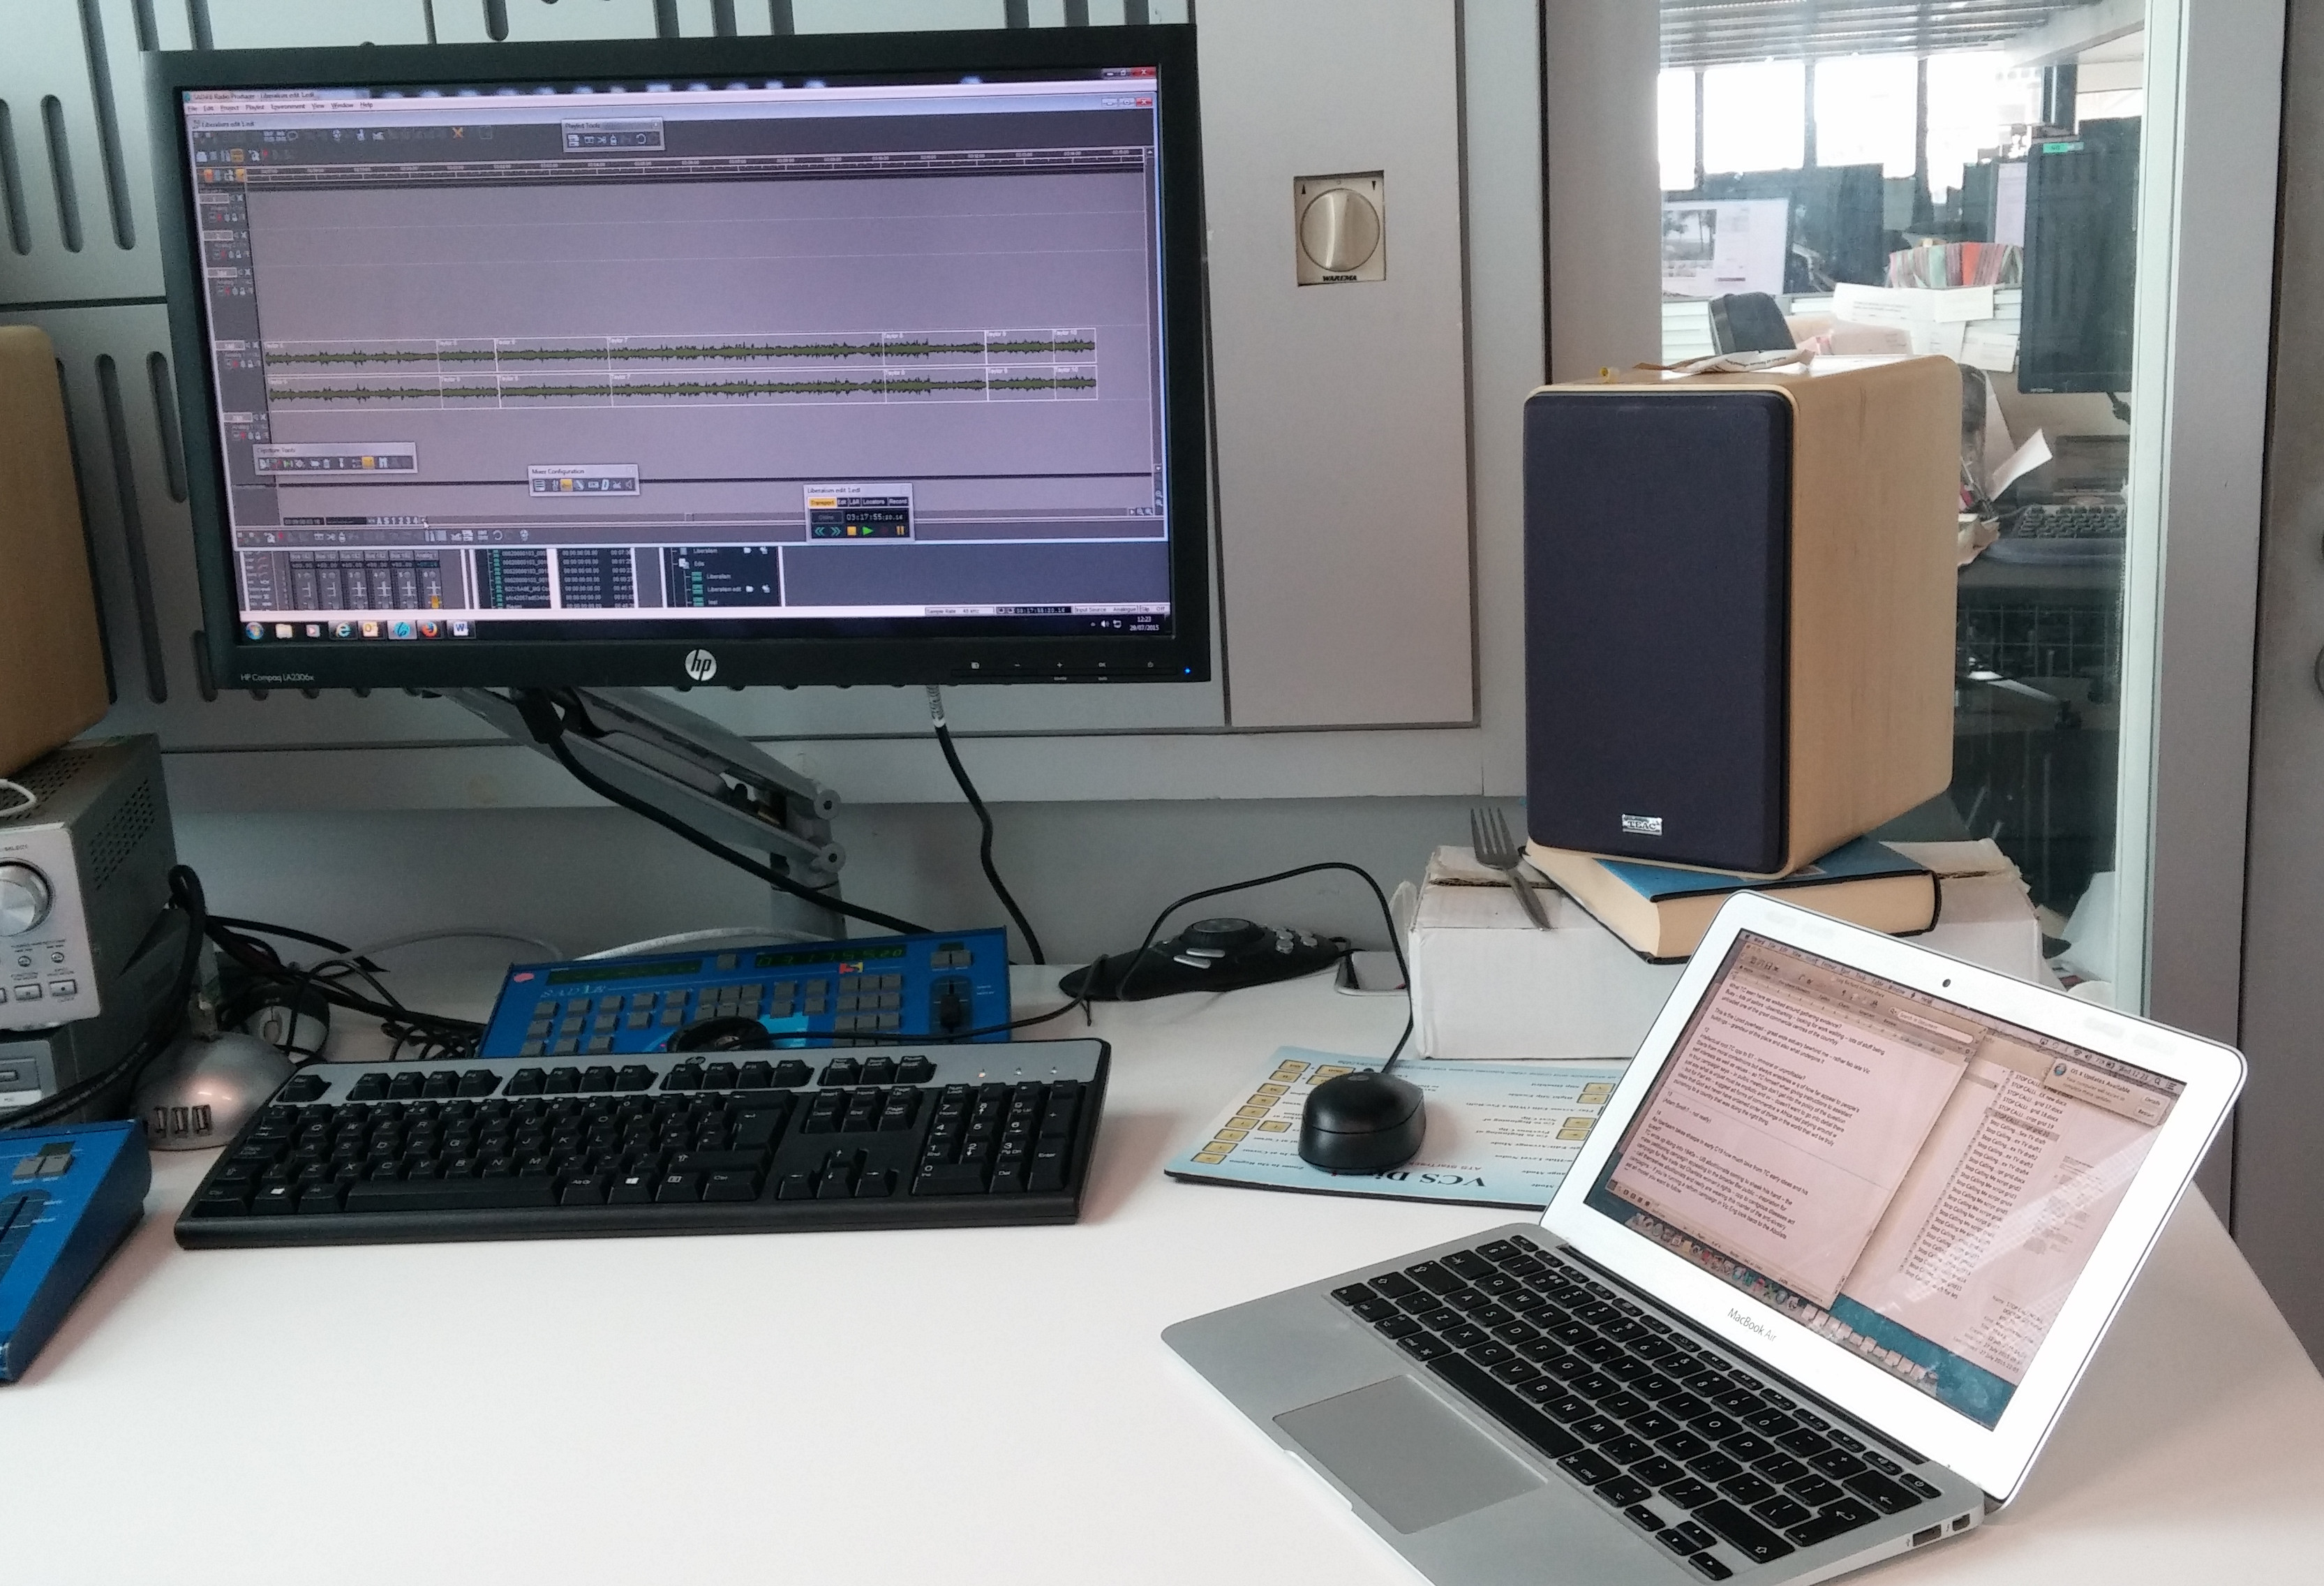
\includegraphics[width=\columnwidth]{figs/phil-desk.jpg}
  \caption{P3 logging interviews with a digital audio workstation on the desktop
    PC and word processor on the laptop}
  \label{fig:desk}
\end{figure}

Logs are usually written by the producer themselves. As they have done the
research and are normally present at the recordings, they can use their memory
to navigate the material and use their experience to quickly determine which
parts are relevant. Some programmes that are under particular time pressure
will use a third-party to create a verbatim transcript of a few interviews
\citep{Baume2015}, but most do not because it is too expensive.

Writing the logs takes a lot of concentration as the producer must listen to
what is being said, work out how it ties in with other contributions and the
story, and make swift judgements on whether it should be used.

\textit{``one of the slightly exhausting things about doing it is the level of
  concentration you have to maintain to make good decisions, remember where
  everything is, what you've got, is kind of strained rather by having to just
  do shleppy tasks like moving the sound and logging interviews''} (P3)

Additionally, many producers find that the open plan office in which they work
is not the best environment for writing logs. For this reason, many choose to
do it away from the office. 

\textit{``I typically do this at home because I find it a much less distracting
  environment. It does require quite intensive concentration so you don't miss
  something.''} (P1)

The high level of concentration required, combined with the repetition of 
typing and listening to the interview again means that producers need to take
regular breaks.

\textit{``it's boring and it's not very easy to be efficient at it [...] when
  I'm normally doing it I'm checking my emails, making a cup of tea.''} (P3)

In the observation, P1 and P3 wrote their logs in Microsoft Word whilst using a
digital audio workstation (DAW) to play the recording (see
Figure~\ref{fig:desk}). P5 reported that they usually followed a similar
process, but did not do any logging during observation.

P4 also did not do any logging during observation, but explained that they
would normally write their logs by hand in a notebook whilst listening on a
portable music player somewhere away from the desk, such as in a caf\'e.

P2 used a different approach. They played the recording in a DAW and used a
keyboard shortcut to create timed markers at any points of interest. By seeing
where the markers clustered, they identified where to make clips, then gave
each of the clips labels. This approach allowed them to focus more on the
audio, but didn't allow them to make any detailed notes.

The exact format of the logs varied between individuals, but they usually
contained a rough transcript of the interview with occasional timestamps and
notes. They reported that this helped them to find important bits in the
recording later on. Each producer has their own syntax, but there are
commonalities.

Timestamps were written on the logs, approximately \textit{``every 30 to 120
  seconds''} (P1) with minutes and seconds in parenthesis: \texttt{(4'20)},
for example.  This allows the producer to navigate to a particular piece of
audio much faster than they would otherwise by narrowing down their search
range.

P1, P3 and P5 would make comments for themselves in the log to help them when
editing. For example, ``\textit{[good to here, dull after]}'' or
``\textit{[trails off 9'30]}''. P1 also used a star rating system to rate the
quality of each point, for example ``\textit{[**** should use this stuff, but
  dramatically cut down]}''.

\textit{``What I sometimes do when I edit are star good bits, and I think
  that's quite a common trait.''} (P3)

Bold highlighting was also used by P1 and P3 to mark bits of the transcript
which are important and worth keeping.

\textit{``what I did was just put in bold the paragraphs I thought were worth
  [keeping]''} (P1)

Every participant that was observed logging played the audio faster than real
time at least once. This allowed them to fast-forward through parts of the
interview that may not be of interest (e.g. discussion in the background)
whilst still being able to listen out for anything they might want to use.

\subsection{Rough editing}
This stage involves extracting audio clips from the recordings which will form
the basis of a draft edit of the programme. If the recording was short and had
been recorded recently, as was the case for P4 and P5, it can be edited without
a log. In this situation, we observed that the producers listened through the
recording using a DAW and pressed a keyboard shortcut to split the recording,
usually at the beginning/end of questions/answers. They then went back and
removed unwanted segments.

If the recording has been logged, the producer will use the log to decide which
parts to select or remove. They use the timestamps written in the log to narrow
down their search area for each clip they extract. However, even with a reduced
search area, the producers find it time-consuming to find the exact start and
end point of each clip using the DAW interface.

In the study, three of the participants (P3, P4 and P5) used SADiE as their
DAW, which is provided to the producers by the BBC. However, the other two
participants chose to use other software packages that aren't formally
supported. P1 used Adobe Audition because they were familiar with the interface
and it was installed on their laptop, unlike SADiE which was only available to
them on a desktop computer.

P2 comes from a television production background and used Apple's Final Cut
Pro, which is primarily a video editor but also includes audio editing
functionality.  Similarly to P1, P2 used Final Cut Pro because they were
familiar with the interface and had it on their laptop. In addition, they
enjoyed being able to import audio directly from video content without having
to use another program to extract the audio first, and being able to use the
video `titles' feature to make written notes.

At the end of this stage, the producer will have clips of their recordings
assembled into a basic structure of their programme in the DAW. This will
normally be about twice as long as the final programme, sometimes significantly
longer (e.g. P5 created 22-hour-long rough edit for a 37-min programme). The
producers then continue to trim the edit down to a manageable length.

\subsection{Fine editing}
The next stage is to add narrative elements, known as `links' to join the clips
together into a storyline. The producer and presenter will write the links
together, using the programme script to collaborate. The presenter records
the links in a studio and the producer then assembles them into the edit.

Once all of the content has been added to the edit, the final stage is to `get
it down to time', adjust the audio volume, and to add any music or
sound effects. The speech is cleaned up by removing redundant noises (e.g.
`umm', `err', `you know') in a process known as `de-umming'. We observed that
many producers brought in an experienced sound engineer to help with any
final complicated editing.  Once the editing is complete, a final version is
rendered to a stereo audio file and added to the radio playout system for
the producer's editor to sign-off.

\section{Study results: New workflow}\label{sec:resultsnew}
This section discusses the results and themes that emerged from the evaluation
of the semantic editing interface. We start by outlining the results of the
usability test (Stage 2) before going into detail on each of the themes that
came out of the observation (Stage 3) and the final interview (Stage 4).
The coding software RQDA was used to identify the themes and to extract
suitable quotes.

%To evaluate the semantic editing interface, participants were observed while
%they used the system to log and rough edit recordings for a programme.
%Although it was designed as an all-in-one solution for putting together a rough
%edit for a programme, participants used the interface in different ways to
%integrate with their existing workflow.

%P3, P4 and P5 used the interface much as designed by using the transcript
%window to read and identify suitable clips, then dragging them across to the
%edit window and exporting the audio.

\subsection{Usability test}
Participants were first introduced to the semantic editing interface through a
usability test (Stage 2). P1 completed the test quickly and without issue,
expressing that it was easy and intuitive. The other four participants
successfully completed the test, but identified a number of minor usability
problems regarding keyboard shortcuts.

Two of the five participants (P2 and P3) kept pressing the space bar to start
and pause audio playback. This may be habitual, as it is a universal keyboard
shortcut in all DAWs. However, this feature was not considered when designing
Dialogger.  Additionally, P2 tried to use word processing shortcuts in the
interface, such as Ctrl+C and Ctrl+V to copy/paste and backspace to delete.

P1, P2 and P4 reached for Ctrl+F to search for a word they were
looking for. Although this feature wasn't explicitly implemented or mentioned in the
training, the functionality was included in the browser. The participants
remarked that it was a powerful tool for navigating the recording.

In conclusion, we found that keyboard shortcuts are more important than we had
considered when designing Dialogger.

%The interface was designed to allow users to copy the text of the entire
%transcript by pressing a `copy' button. Four of the five participants
%intuitively selected the text before pressing the copy button.  P2 expressed a
%preference to use Ctrl+C and Ctrl+V shortcuts to copy and paste text, rather
%than a drag-and-drop gesture.  Additionally, P2 said they wanted to be able to
%remove selected text by pressing backspace, or to export only selected text.
%Future versions should
%consider allowing users to apply actions only to selected text.

%Three of the five participants (P2, P3 and P5) couldn't remember the action to
%correct a word (double-click). Two of them (P2 and P3) right-clicked the text
%and looked for an option in the context menu.

%P2 confused about double waveform

%\section{New workflow}
%Following the usability study, participants were observed using the prototype
%interface to complete a common production task and interviewed about it
%afterwards. This section documents the findings.

\subsection{Navigation and editing}
Participants reported that having the transcript available in the semantic
editing interface allowed them to read and search the recordings much faster
than they normally would with a waveform.

\textit{``with having a transcript you're able to immediately scan through it
  10/15 times faster. Maybe that's an exaggeration but it feels ten times
  faster''} (P1)

The transcripts also allowed the participants to quickly cross reference what
was said in various interviews without having to listen through multiple times.

\textit{``where I'm picking shorter clips, making a point and moving on or I'm
  developing an argument between different people and cutting between them, it
  feels a lot more easy to construct that `on paper' than what I'm currently
  doing''} (P2)

%\textit{``If it's a shorter thing I'll bang it straight into SADiE and start
  %editing down to find the wheat from the chaff''} (P4)

Being able to click on a word to navigate to that point in the audio also
enabled the participants to use visual search to quickly find and listen to
bits they were looking for.

\textit{``you can do that with your eyes even quicker - zone straight in on the
  bits and that click to go  `that bit', `that sentence there', `that word
  there' ''} (P4)

Participants reported that editing with a transcript was primarily useful when
working at the sentence level. When the granularity of editing involves
removing individual words, `umm's or breaths, they said that the DAW software
is much better suited to these tasks. This supports our design decision to
integrate with DAWs.

\textit{``the real editing work actually happens after this has passed its main
  point of usefulness''} (P3)

%\textit{``I was using some interviews, some contributors recorded on one
  %ocassion, but across several programmes, several episodes in a series, or for
  %several different stories.''} (P4)

%\subsubsection{Navigation speed}

%\textit{``it took me 15 mins to read 35 mins and not just read, but read and mark
  %up''} (P2)

%\subsubsection{Time since interview}

%\textit{``you're kind of doing a paper edit on the basis of having recently
  %heard the audio''} (P3)

%\textit{``a lot of that guesswork was coming from the memory of being there at
  %the recording... realising which bits were the questions from the
  %presenter and which bits were answers.''} (P2)

%\textit{``I know I've got a doc coming up in six months time, so I'll ask them
  %some questions for that. Now then in six months time I can't remember what
  %the answer was''} (P4)

%The primary benefit of reading over listening is that you can quickly scan
%ahead and jump around with your eyes, whereas listening can only be done at a
%fixed pace. 



\subsection{Transcript accuracy}
When using the semantic editing interface, editing decisions are based
on an automated transcript which is only partially accurate. However,
participants suggested that the transcripts were, generally speaking,
sufficiently accurate for their purposes.  \citet{Whittaker2004} found that
imperfect transcripts were sufficiently accurate for voicemail editing. These
results show that this finding could also apply to radio production.

\textit{``It's clearly not 100\% in word recognition but I'm feeling it's
  certainly good enough for my rough cut purposes at this point''} (P2)

If the recording being edited was made recently, the producer can use their
memory of what was said to make sense of the inaccuracies in the
transcript.

\textit{``Both these interviews [being edited] are relatively recent so I have
  it reasonably in my mind what they've been saying. I was able to read roughly
  what there was - `okay that's that question', `I know what was in that
  question' ''} (P1)

Although most of the producers we observed only used the transcript to navigate
and edit the audio, some were interested in correcting the transcript so it
could later be shared or published.

\textit{``I'm probably posting transcripts for the whole interview. So I do
  need to go through and correct''} (P4)

Clearly, the more accurate the words in the transcript are, the less work has
to be done to correct it.

\textit{``The closer it can be to the point where you don't have to clean it up
  the better obviously, and that's quite significant honestly, that's my only
  qualm''} (P3)

%Sometimes a word is commonly mistranslated throughout the transcript, so
%providing an easy way to fix that would be a useful addition.

%\textit{``Something that would be even better is Ctrl+H  replace function''}
%(P3)


%\subsection{Speaker diarization}
%One disadvantage of working with transcripts is that you can't hear which
%person is speaking when.

%\textit{``if you can't see who's speaking - that's a disadvantage''} (P3)

%Speaker diarization technology \citep{AngueraMiro2012} can be used to try and
%identify where different people are talking. The prototype included a
%rudimentary system that attempted to distinguish speakers and guess their
%gender, however it tended to significantly overestimate the number of speakers
%which caused some difficulty. 

%\textit{``It was distracting if anything, partly because I was trying to guess
  %who was which at certain points''} (P2)

%However, in many situations the participant could tell who was who from what
%they were saying.

%\textit{``It's reasonably clear to me who's asking the questions, but actually
  %[speaker diarization] is helpful''} (P1)

%During the study it was discovered that many producers record in stereo and use
%the waveform to see where people are speaking.

%\textit{``I always pan the presenter on one side and the contributor on the
  %other so I can see where the questions are''} (P5)

%This workaround could be exploited to improve the performance of a more
%advanced speaker diarization system.

\subsection{Annotation}
%Before creating any clips, P1 immediately copied the transcript text into Word
%in order to allow them to make annotations.

%The WAVs were then imported into the DAW
%by dragging and dropping them from the file system.

%In the observation stage, it was identified that annotation is an important
%part of the production process that was missing from the prototype.
P1 and P3 copied the transcript text from the interface into MS Word. They
reported that they did this because there was no annotation functionality
available within Dialogger.

They inserted paragraph breaks, added notes after each paragraph, and
highlighted desired parts of the transcript in bold. Once the transcript was
annotated in MS Word, they went back to Dialogger, found the parts of the
transcript they wanted by scrolling though the text, then dragged and
exported each clip individually as a .wav file.

\textit{``it would be better to take raw lumps of transcripts and plonking them
  in Word because Word has higher functionality than this''} (P3)

Producers are very familiar with the MS Word interface so a later version of our
system could seek to provide a similar interface. This would allow producers to
make annotations in the same way they do already.

\textit{``With text editing, the reflexes are very much Microsoft Word''} (P4)

The most basic feature that could be added is highlighting, which is often used
to note parts of interest

\textit{``If you just put a little star or underline or something simple to
  mark things, that would be a big gain for a small change''} (P3)

%\textit{``sufficient to find the bits of the audio you want to use and to make
  %sense to the presenter.''} (P3)

%\subsubsection{Star rating}

%\textit{`` I just gave myself a detailed breakdown of what was said in the
  %interview with timecodes at questions or major new points and a slightly
  %arbitrary scoring system to say 'that's really good stuff and must get in'.
  %''} (P1)

\begin{figure}[t]
\centering
  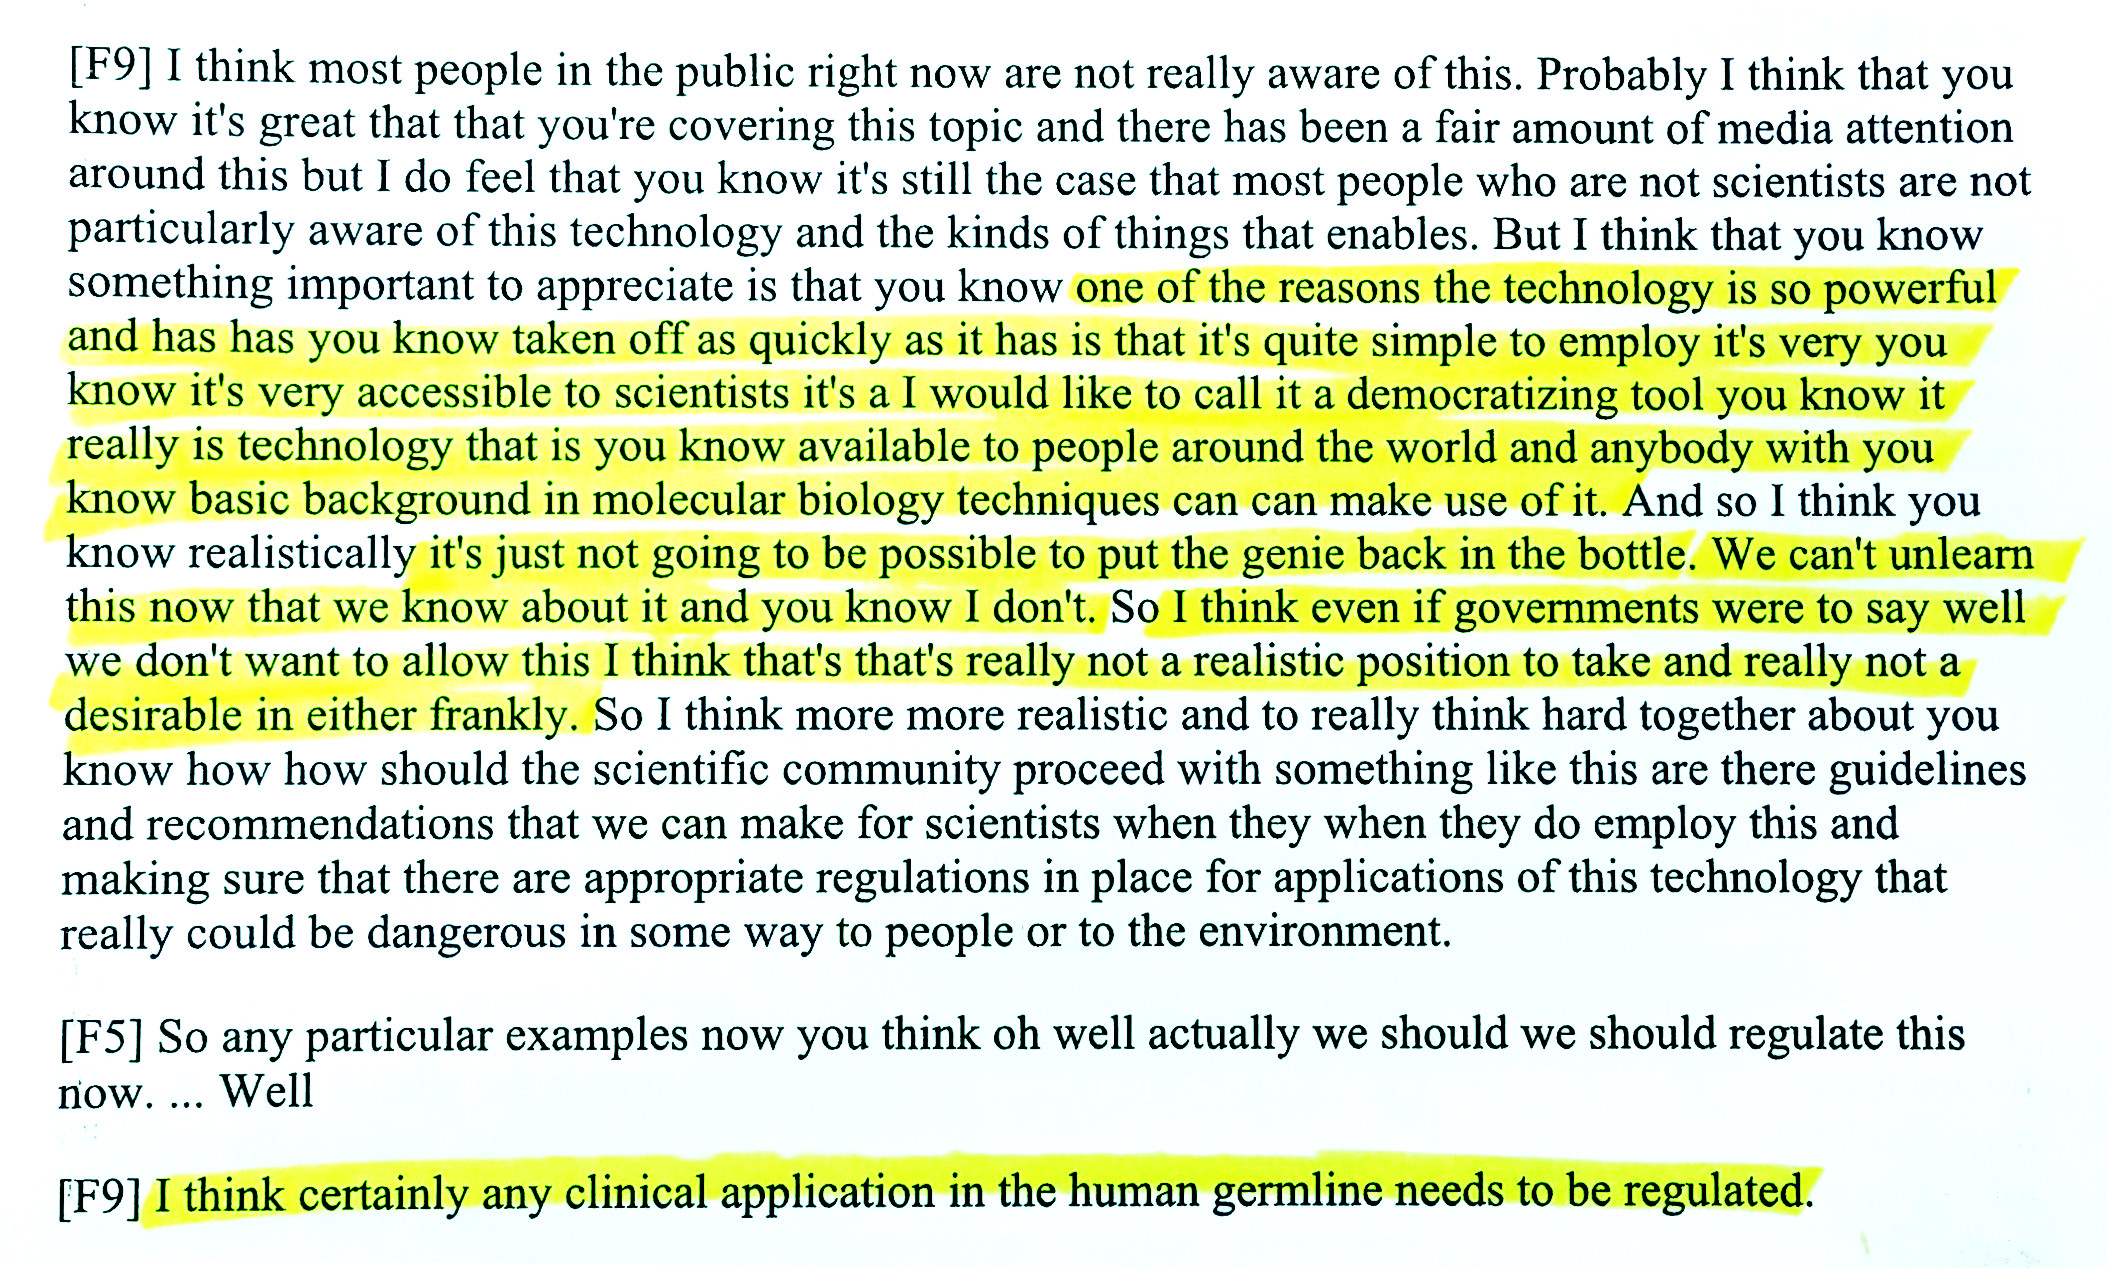
\includegraphics[width=\columnwidth]{figs/highlighting-cropped.jpg}
  \caption{P2 using a highlighter pen with a printout}
  \label{fig:highlight}
\end{figure}

\subsection{Paper}
In the observed task, after uploading their recording, P2 immediately printed
the transcript and read through it on paper so that they could work away from
the screen.

\textit{``I'd prefer to do it on page than on screen. Just easier on my
  eyes.''} (P2)

Producers reported that working on paper allowed to be productive outside of
the office, such as during their commute.

\textit{``What would be really useful would be to [...] take it away (say when
  I'm on the train going home) and I would paper edit the bits that I need''}
(P5)

%\textit{``In the office there's so much pressure and you're always doing stuff. When you
 %can step away from that, have a long commute, I can think''} (P5)

Additionally, working on paper allows them to work anywhere as it does not
require electricity.

\textit{``It's highly portable. It doesn't require any power.''} (P2)

P2 used a highlighter pen to select the desired parts of the recordings (see
Figure~\ref{fig:highlight}).  After highlighting all the pieces they wanted,
they then used the Ctrl+F text search to find the highlighted words in the
semantic editing interface.  The search feature was not explicitly included in
the editing interface, but was included in the web browser so was discovered by
some participants.

\textit{``it allowed me to get to clips very quickly from a reference point on
  a printed transcript''} (P2)

However P2 noted that having timestamps on the printout would be a faster
way of achieving the same thing.
Once they had found and clipped all of the highlighted parts in the semantic
editing interface, they exported the clips into SADiE.

Another participant explained that for an upcoming programme, they were
planning to print out transcripts from the semantic editing interface to help
them collaborate with their presenter.

\textit{``we're just going to go through it with a pencil and paper, with a
  printout, and highlight the bits we want and cross out the bits we don't.''}
(P4)

\subsection{Listening}
Part of the appeal of having a transcript is that it frees the user from
listening to the audio in real-time. It also allows users to work on paper,
away from any electronic devices. However, disconnecting the audio from the
text fundamentally changes the production process.

\textit{``Radio is made with your ears. You'll never get away from that fact
  that you need to listen''} (P4, also P2, P3, P5)

The criteria for deciding whether a piece of audio is good enough to use in a
programme is not just about what was said, but how it was said. Making
decisions on whether to keep/lose something without listening to it isn't
desirable.

\textit{``How people say things is very important and I wouldn't want to lose
  that totally.''} (P5)

There was also concern that parts which sounded great but didn't come across
as well in the transcript may have been overlooked.

\textit{``I was anxious it might not have sounded as good as it read, or that I
  might be missing bits that sounded great ''} (P2)

In the old workflow, participants occasionally played the audio faster than
real time, but that feature was not included in Dialogger.
Several of the participants noted that they would like to have this
feature added.

\textit{``it's a little bit annoying that there's no facility for that.''}
(P2)

Although faster than real time playback normally reduces intelligibility, this
would be less of a problem if the transcript was available \citep{Ranjan2006}.
This would open the possibility for playback speeds faster than are currently
possible, allowing producers to listen to content much more quickly.

\textit{``you do still need to listen through, even though you've got the text.
Therefore, it would be optimised if we could listen through quickly''}
(P4)

As listening is an important part of the production process, text should remain
linked to the audio wherever possible to allow multi-modal interaction. Once
the link is broken, re-linking the two together can be costly.

%\subsection{Interface design}
%The semantic editing interface was designed so that the user could drag and
%drop selected clips into an edit window. Although this works well for picking
%out short clips, user encountered issues when trying to select and use long
%clips as the edit window quickly filled up.

%\textit{``I found the interface quite clunky for pulling out big chunks of
  %audio.''} (P5)

%Users worked around the problem by dropping new clips between old ones, then
%re-ordering the new clip to the bottom of the list. One suggested fix was to
%have a button to append a clip of the selected text to the edit without having
%to drag and drop.

%\textit{``once you've selected on the left hand side [...] it would go to the
  %bottom of the queue, that would be a useful way of moving stuff from left to
  %right for pulling highlight clips''} (P2)

%Selecting very large amounts of text with a dragging motion also proved tricky,
%so it was suggested that clicking whilst holding shift (like in word
%processing) could fix this.

%\textit{``Just being able to hold shift and use the cursor. Selecting the text
  %was a little bit index finger intensive.''} (P4)

%Although the semantic editor is set up to select good bits, a lot of the
%participants also wanted to get rid of bad bits.

%\textit{``What you need to do is [...] to get rid of the gubbins of me talking
  %to presenters and mistranslating''} (P3)

%Some were also interested in having cut functionality that would remove the
%selected clip from the original recording. This would ensure that it can't be
%used twice.

%\textit{``You could even go further in the spirit of what it is which would
  %being able to cut and paste, delete''} (P4)

%Not all of the participants agreed though.
%\textit{``it wouldn't be something I'd be aching to be introduced''} (P1)

%\subsubsection{Stage of usefulness}

%\textit{``The transcript is useful at a later stage in the production process
  %when I've cut my programmes, when I want to export clips to the news. When I
  %need to compile a final script for a presenter''} (P2)


%\subsubsection{Quantity}

%\textit{``We've got about six hours of audio for a one hour programme, and it's
  %all just one-on-one interviews''} (P4)

%\textit{``you've got to find the right bit which is burdonsome and annoying
  %when you've got 20 interviews to do''} (P1)

%\subsection{Export}

%Stuff on export and integration

%No gaps in WAV

%\subsection{Export}
%Each participant differed in how they exported the
%content.

%P5 made a list of all the clips they wanted for the programme before exporting
%them into SADiE.  P4 made clips for three different programmes from a set
%of eight recordings. They did this by making a list of clips for one programme
%then exported them into SADiE before moving onto the next programme.

%P3 took a different approach by exporting each clip individually as a .wav file
%which they renamed.  Additionally, P3 copied the text from each clip into the
%script for their programme. They then inserted paragraph breaks between
%questions and answers, and highlighted the questions in bold so that they could
%easily identify them.

%P4 queried whether it would be possible to identify which parts of the
%recordings had already been used, so that they wouldn't be re-used in other
%programmes.

%\subsection{TV}

%Two participants suggested that text-based editing would be equally, if not
%more, useful for TV production. P2, who formerly worked in television, said
%that their workflow already followed a similar pattern. 

%\textit{``If I was making a TV show this is what I would do. I'd effectively
  %print [a transcript], read, highlight, pull a collated collection of those
  %clips or number then, then write a draft script that combined everyone's
  %interview highlight clips that I thought were relevent for telling the
  %story.''} (P2)

%The costs involved in producting TV content are much higher than radio, so
%there is a greater financial incentive in streamlining the process.

%\textit{``There's an advantage to paper edit in TV because the assemblage
  %process takes longer and you might decide you don't need particular bits of
  %archive you thought you did and [save on] transfer costs.''} (P3)

% ran out of space

\subsection{Follow-up}\label{sec:followup}
After the interviews and observations were complete, the participants were given
access to Dialogger for a further month (Stage 5). During this time their
actions were logged electronically and they were emailed each week to ask which
features they found useful, or were missing. P3 was unavailable immediately
after the study, so could not take part in the follow-up stage.

Most of the comments received in the follow-up stage were already picked up by
the first part of the study. In the remaining comments, all of the participants
said they enjoyed being able to use the semantic editor outside of the office
and at home. Some reported that they had issues uploading content with their
slow network connections, and P2 suggested that allowing multiple simultaneous
uploads would allow them to leave it running overnight.


\section{Study results: Metrics}\label{sec:resultsmetrics}
\subsection{Time}

\begin{figure}
\centering
  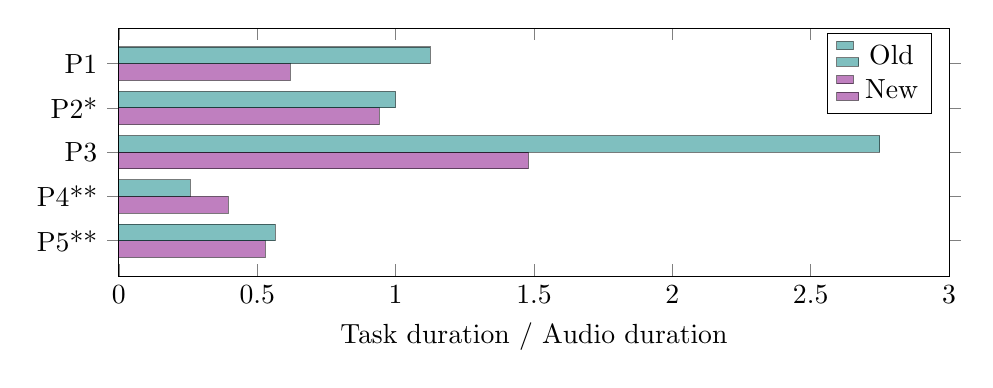
\begin{tikzpicture}
  \begin{axis}[
      width=\columnwidth,
      xbar=0pt,
      bar width=6pt,
      xlabel=Task duration / Audio duration,
      y=16pt,
      xmin=0,
      xmax=3,
      enlarge y limits=0.2,
      symbolic y coords={P1,P2*,P3,P4**,P5**},
      ytick = data,
      y dir=reverse,
      reverse legend,
      ]
  \addplot[fill=violet, opacity=0.5] coordinates {(0.619,P1) (0.941,P2*) (1.48,P3) (0.395,P4**) (0.529,P5**)};
  \addlegendentry{New}
  \addplot[fill=teal, opacity=0.5] coordinates {(1.125,P1) (1.0,P2*) (2.75,P3) (0.258,P4**) (0.565,P5**)};
  \addlegendentry{Old}
  \end{axis}
  \end{tikzpicture}
	\caption{Time taken to complete the observed task for each workflow, compared
    to the original audio length. Lower is better. *P2 logged their material on
    paper. **P4 and P5 did not do any logging.}
  \label{fig:time}
\end{figure}

The time taken to complete the observed tasks was recorded (see
Figure~\ref{fig:time}). As different recordings of different lengths were used
for the old and new workflows, the times are reported relative to the length of
the audio. In all cases, the producers were able to run the speech-to-text
processing as a background task so this was not included in the calculation.

The variability in the timings was due to the workflow of the individual
producers. P4 and P5 did not do any logging, so started editing the audio
immediately. In this case editing the audio using the semantic editor was not
any faster than the existing method and in the case of P4 was slower.
The participants noted that the overhead of having wait for a transcript is
too much if the editing task is only small.

\textit{``If it's a quick ten minutes with three questions, you don't need to
  bother''} (P3, also P4 and P5)

P2 did go through a logging stage, but did this by printing out the generated
transcript and using a highlighter pen to select the bits they wanted. This
meant that they had to go back and repeat this process using the semantic
editor interface, which slowed them down. Despite this, the new process was
marginally faster.

P1 and P3 used Dialogger as designed by logging and editing their material
using the semantic editing interface. The length of their interviews were also
much longer, so the benefit of text-based navigation and editing was more
apparent. In this case, the producers rough edited their material nearly twice
as fast as their existing workflow.

In summary, there is little speed benefit when the recording is short and
logging is not needed, but when Dialogger is used for logging
and rough editing on longer recordings it is approximately twice as fast as the
current method.

\subsection{Cognitive load}


%\begin{table}
  %\centering
  %\begin{tabular}{ r | c c c c c | c }
    %& P1 & P2 & P3 & P4 & P5 & Mean \\
    %\hline
    %Mental demand   & -5  & -9  & -2  & 5   & 4 & -1.4 \\
    %Physical demand & 0   & 4   & 0   & 13  & 0 & 3.4 \\
    %Temporal demand & -1  & 4   & -5  & 4   & 1 & 0.6 \\
    %Performance     & -2  & 7   & 0   & 2   & 5 & 2.4 \\
    %Effort          & -1  & -7  & 7   & -4  & 2 & -0.6 \\
    %Frustration     & -12 & 1   & -3  & 2   & 5 & -1.4 \\
    %\hline
  %\end{tabular}
  %\caption{Difference in NASA-TLX results between the old and new workflows.
    %Negative results indicate that the new workflow is better.}
  %\label{tab:tlx}
%\end{table}

After completing both tasks in the observation, the participants were asked to
rate both the old and new workflows using the raw NASA-TLX metrics
\citep{Hart1988}.  The results are shown in Figure~\ref{fig:tlx}.

With only five participants and marginal differences, it is not possible to
draw any conclusions about cognitive load from these results.  They indicate
that Dialogger requires slightly less effort and mental demand, and is less
frustrating. However it is considered more physically demanding, temporally
demanding and scores lower in performance.

%To put these results in context, we must look at what the
%participants said in the interviews.

\begin{figure}
\centering
  \begin{tikzpicture}
  \begin{axis}[
      width=0.8\columnwidth,
      height=0.8\columnwidth,
      bar width=6pt,
      xbar=0pt,
      xlabel=Mean TLX value,
      y=16pt,
      xmin=0,
      xmax=100,
      enlarge y limits=0.15,
      symbolic y coords={Frustration,Effort,Performance,Temporal demand,Physical demand,Mental demand},
      ytick=data,
      legend pos=east,
      legend style={at={(1,0.5)},anchor=east},
      reverse legend,
      ]
  \addplot[fill=violet, opacity=0.5] coordinates {(44.5,Frustration) (53,Effort) (41,Performance) (51.5,Temporal demand) (48,Physical demand) (51,Mental demand)};
  \addlegendentry{New}
  \addplot[fill=teal, opacity=0.5] coordinates {(48,Frustration) (54.5,Effort) (35,Performance) (50,Temporal demand) (39.5,Physical demand) (54.5,Mental demand)};
  \addlegendentry{Old}
  \end{axis}
  \end{tikzpicture}
  \caption{Mean NASA-TLX results for each system. Lower is better.}
  \label{fig:tlx}
\end{figure}

\subsection{Follow-up usage}
The logs from the interface were analysed to see how the participants used
Dialogger during the follow-up stage of the study, to discover which features
were being used, and for how long.

All of the participants continued to use the semantic editor of their own
accord as part of their work. The total time spent by the four remaining
participants (P1, P2, P4, P5) using Dialogger in the follow-up period was 23 hours
and 58 minutes.  Over 14 hours of those were from P2, with P4 using it for 5
hours, P1 for 3 hours and P5 for 20 minutes.

\begin{figure}
\centering
  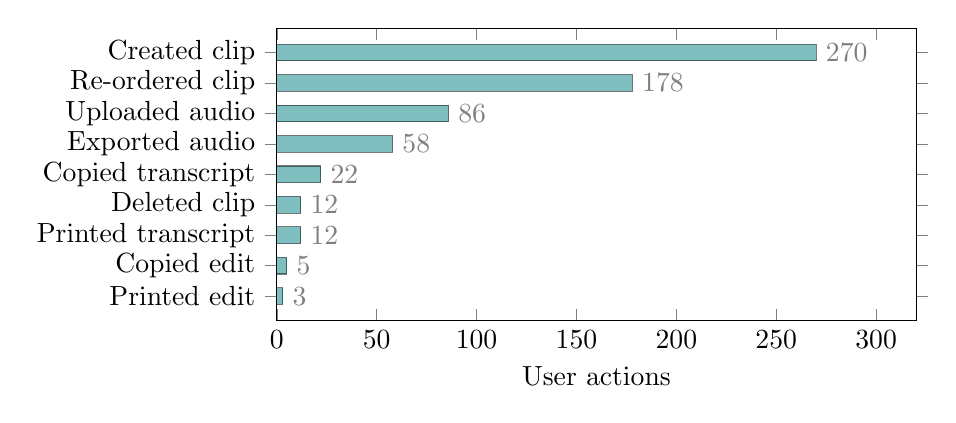
\begin{tikzpicture}
  \begin{axis}[
      width=0.8\columnwidth,
      %height=0.7\columnwidth,
      bar width=6pt,
      xbar=2pt,
      xlabel=User actions,
      y=11pt,
      xmin=0,
      xmax=320,
      symbolic y coords={Printed edit,Copied edit,Printed transcript,Deleted clip,Copied transcript,Exported audio,Uploaded audio,Re-ordered clip,Created clip},
      ytick=data,
      nodes near coords,
      ]
  \addplot[fill=teal, opacity=0.5] coordinates {(3,Printed edit) (5,Copied edit) (12,Printed
    transcript) (12,Deleted clip) (22,Copied transcript)
    (58,Exported audio) (86,Uploaded audio) (178,Re-ordered clip) (270,Created clip)};
  \end{axis}
  \end{tikzpicture}
  \caption{Count of logged user actions during follow-up}
  \label{fig:actions}
\end{figure}

Figure~\ref{fig:actions} shows that over 80 recordings were uploaded and over
50 audio edits were exported. The figure also shows that copying the transcript
was more popular than printing it.

Users could navigate the content by either clicking on the waveform or by
clicking on a word in the transcript. In the interaction log, over 98\% of
navigation actions were executed by clicking on a word, which shows a clear
preference for navigating by text.

%\section{Implications}

%Remove as well as take away

%Annotation is import. Need to include word processing features

%Paper is still used, portable and easy on eyes

\section{Discussion}\label{sec:discussion}
% Others didn't test properly, we did
Previous work on transcript-based media interfaces introduced a range of novel
features for semantically navigating and editing audio and video content.
\citet{Whittaker2004} showed that for voicemail content, semantic editing using
automatic transcripts was faster and as accurate as waveform-based editing.
\citet{Casares2002}, \citet{Berthouzoz2012} and \citet{Rubin2013} all created
similar systems for audio and video production, but they used perfect
transcripts and did not perform any formal studies on the semantic editing
features. In this paper, we presented a semantic speech editor that was
designed specifically for radio producers based on the results of a pilot
study. We studied the existing workflow and evaluated the impact of the
semantic editor through a qualitative study of five professional radio
producers.

% Logging and rough editing is boring
We found that for production of factual radio programmes, a significant amount
of time is spent `logging' speech recordings by transcribing them by hand and
making notes. This process helps the producer to select the best bits of their
material and to structure the narrative of their programme. After logging,
producers create a rough edit by using an audio editor to pick out each piece
of audio they want, guided by the timestamps in their notes. However, these
processes take a long time, require concentration, and are considered to be
boring and tedious.

% Our system was much faster, so frees up their time for other things
Our semantic editing system `Dialogger' introduced automatically-generated
transcripts, which meant that the participants could log their recordings much
faster.  Additionally, the interface allowed them to edit the audio directly
from the transcript, bypassing the rough edit stage, and saving additional
time. Freeing-up this time would allow the producers to concentrate on more
valuable activities such as background research, finding contributors, or
recording additional material. In turn, this could have the potential to
improve the editorial quality of the programme.

% Most of the benefit is from the transcript itself, but how much?
In our experiment, the automatic transcription and the editing interface were
tested as a whole. However, many participants suggested that most of the
benefit derived from the system came from the automatic transcription. A future
study could test these aspects separately to investigate the proportional time
saved by the transcription compared to the interface itself.

% The transcripts aren't perfect, but they're good enough to edit when you can
% listen
As the transcripts were automatically-generated, approximately 16\% of the
words were inaccurate. Despite this, most participants found them to be
sufficiently accurate for their purposes, which supports the findings from
voicemail editing \citep{Whittaker2004} and voice-based discussions
\citep{Sivaraman2016}. 

% Even if the transcript is perfect, producers still need to listen
In theory, if the transcripts were perfect, it would be possible to rough cut
recordings without having listened to them. However, a verbatim transcript
cannot tell you whether something was said seriously or in jest, or about
emphasis, cadence, intonation or background noise. Therefore, an interface that
allows users to edit speech based purely on the transcript carries the risk of
creating poor quality results. It is important for such systems to make it easy
for users to listen to parts of the transcript so they can determine the
quality of the audio they are editing.

% Transcripts need correcting to be readable on their own
Although the automatic transcripts were considered good enough to edit with,
the producers often had to listen to parts of the recording to make sense of
them. If the transcripts are to be used independently of the audio, the
producer must have an easy way to fix the mistakes. Rather than make the user
type out each replacement word, this process could be aided by allowing them to
select alternative words that were rejected by the speech-to-text system.

% Many producers like working on paper, but need to listen to make sense
Despite the importance of listening, many producers like to work on paper.
Participants said that they enjoyed being able to work away from the desk, that
it was easier on their eyes, and that it was easier to collaborate with others
using printed documents. However, when transcripts are printed, the timing
information which links the words to the audio is lost. It would be feasible 
to develop a system for moving between paper and the screen which could
retain this information, but no such existing system could be found.

% Annotation helps the producer to mark their favourite bits
The role of the transcripts is ultimately to help the producer pick which bits
of audio to use in their programme. To achieve this, they use annotations to
mark and rate segments of the transcript. This functionality has not been
considered in any previous semantic editing systems, but we found it to be an
important feature which participants went out of their way to replicate.

In creating and testing Dialogger, we found that there was demand for semantic
editing in radio production. This was backed up by the continued use of the
system during the follow-up period, which was unprompted.
During the study, many of the radio producers reported that a similar
transcript-based workflow exists in television production. Due to the high
costs of video editing, transcripts are often used to make editorial decisions
before editing begins. It would be interesting to see if a semantic video
editor would bring similar benefits to a television production workflow.

% What did you learn from making the system?

% What does this tell us about these kinds of systems?
%- Mature enough to be used in professional practice


% How does this impact the workflow?

% How does this impact the job role?


% Television


% How does this impact the nature of programme making


%CONTIBUTIONS COMPARED TO OTHER WORK

%Logging helps producers to recall what was said in interviews and to structure
%and cross-reference

%Logging takes a long time, requires concentration and is boring.

%Producers annotate the logs with timestamps, notes, highlighting and star
%ratings.

%Word is used and preferred for making annotations

%Navigation using a transcript is considered faster

%There is a desire to listen to the audio faster than real time

%The transcript is accurate enough to do a rough edit

%A more accurate transcript would be beneficial

%The transcript interface is not needed for short recordings or fine editing

%Drag and drop clipping didn't work very well as it's hard to select long bits

%There is a desire for cut and delete functionality

%Working on paper is desirable

%Television could also benefit from this approach

%Need to listen to the audio

%Task completed up to twice as fast with the new system when including logging

%Participants continued to use the prototype after the study

\subsection{Outcome}
Based on the results of this work, we developed the prototype further to add
support for video editing and to take into account the feedback from the
producers in our study.  We handed the prototype over to a development team at
the BBC who have now turned it into an officially supported production tool. We
hope that this will allow producers from around the BBC to use the tool as part
of their normal workflow.

\subsection{Summary of main findings}\label{sec:findings}
%used a pilot study to identify an opportunity to use automatic transcripts of
%dialogue with synchronised audio to connect two previously separate activities
%in radio editing. This had mixed results as shown by the weak stats but more
%positive comments. It exposed some important missing functions like annotation
%and the importance of paper. The exercise also seems to have resulted n the
%first published study of documentary radio production.

% start with a summary and then extend each element at greater length

\paragraph{There is demand for semantic editing in radio production}
In the follow-up stage of the study, all of the participants continued to use
the semantic editing interface of their own accord as part of their production
workflow. This result demonstrates that they find the interface beneficial to
their practice. The interface has also been developed into a supported
production tool which also demonstrates that there is a business case in making
this available to production staff.

\paragraph{Semantic editing is faster for long recordings}
For editing short audio content ($\sim$10 mins), or when editing without
logging, we found that there was no speed benefit in using semantic
editing. However, logging and rough editing longer recordings using the
semantic editing workflow was completed up to twice as fast as the existing
workflow. Participants also commented that the semantic editing system felt
much faster to use and allowed them to quickly search and cross-reference the
material.

\paragraph{Automatic transcriptions are sufficiently accurate}
The participants in the study used automatically-generated transcripts to
navigate and edit the audio. Even though the transcripts had a word error rate
of approximately 16\%, they were found to be sufficiently accurate for the
purposes of radio production.  This supports similar findings about semantic
editing of voicemail content from \citet{Whittaker2004} and of voice-based
discussions from \citet{Sivaraman2016}. However, the more accurate
the transcripts are, the better.

\paragraph{Annotation features are important}
Participants annotated their logs with timestamps and notes, and used star
ratings and highlighting to indicate important parts of their recordings. As
this functionality was not included in the semantic editing interface, some
participants imported the transcripts into MS Word to allow them to make these
annotations.  This demonstrates that annotation is an important feature to
include in such systems.
%This broke the connection between the audio and the text.
%These annotation features could be added to the semantic editing system which
%would allow the audio and transcript to remain linked.

%\subsection{Drag-and-drop doesn't work}
%The interface was designed so that users could select desired pieces of content
%using a drag-and-drop technique. This design worked well for short clips, but
%could not handle long clips. In addition to selecting content they did want,
%participants were also interested in removing content that they didn't want. 
%Enabling word processor style editing like cut, copy and paste would give the
%users more freedom.
%%TODO SO...

\paragraph{Producers want to work on paper}
The participants often used paper to read and annotate their scripts and logs
because it was easier on their eyes, helped them to collaborate and allowed
them to be productive away from the desk, such as in caf\'{e}s and on trains.
During the study, one participant printed the transcript from the semantic
editing interface and worked on paper, even though this meant having to go back
to find and create the desired clips.

%went out of their way to edit on paper by printing and
%highlighting the transcript.  Being able to move between the screen and paper
%would bring the benefits of paper working and allow producers to use their time
%more efficiently.

\paragraph{Listening is important}
Finally, participants pointed out that ``radio is made with your ears''.
Editing decisions are based not only on what is said, but how it is said. This
emphasises the importance of a multi-modal interface, which combines the
efficiency of text-based working with being able to quickly listen back to the
audio.  Enhancing this with faster than real time listening would allow
users to review material at much faster speeds than they do already
\citep{Vemuri2004}.


\section{Conclusion}\label{sec:conclusion}
Semantic editing of speech has direct applications in professional audio
production, but previous studies of such systems were informal and used amateur
participants. We developed a semantic speech editing system based on the
results of a pilot study of radio production, and conducted a formal user study
of the system with five producers at the BBC.  We used speech-to-text to
generate transcripts, which were accurate enough to allow the producers to
rough-edit their recordings up to twice as fast as their current method.
During the study, we discovered that annotating the transcript is an important
part of the editing process, and that producers enjoy working on paper.
Although it is possible to use these systems to edit audio using only a
transcript, we found that it cannot replace listening to the audio. After the
study, the producers continued to use the system, which has since been
developed into a supported BBC production tool after receiving investment.

\section{Future work}
One of our findings was that producers want to be able to work on paper. In
order to facilitate this, we are currently working with a digital pen
manufacturer to develop a semantic editing system that would allow producers to
edit the audio by annotating a printed transcript. 

%As the semantic editing tool becomes part of the normal production workflow, we
%will closely monitor its usage and attempt to measure its impact. We will do
%this by building in metrics and setting up a working group to receive regular
%feedback directly from users.

We found that semantic editing was faster for long recordings, but it would be
interesting to investigate how long a recording needs to be before the benefits
of semantic editing outweigh the costs. Additionally, it is unclear how much of
the speed benefit comes from automatically generating the transcript, and how
much comes from the editing interface.

%In future work, we plan to improve the semantic editing interface by adding
%faster than real time playback, and moving closer to a word processing style
%design that includes cut, copy, paste, delete, undo and annotation features.

%We will also be investigating whether a
%similar system can be achieved on paper using digital pen technology.

Now that our system has been developed into a supported production tool, we
will monitor its progress and record metrics to track its usage. As the
system now includes support for video editing, it could be used to investigate
the benefits and challenges of semantic editing for television production, and
contrast it with those of radio production.

%Semantic speech editing systems allow users to navigate and edit speech-based
%audio or video content using a transcript-based interface.  Previous studies
%have demonstrated the potential of this approach for a variety of applications,
%however the evaluations have all been in a laboratory setting and have mostly
%been informal.  In this paper, we presented the first evaluation of semantic
%speech editing in an uncontrolled environment.

%We conducted a qualitative study of five radio producers at the BBC to discover
%how programmes are made, and to evaluate our semantic editing system. The study
%found that current radio production practice involves spending a lot of time
%logging and rough editing interviews, which is lengthy, requires concentration
%and is considered boring.

%Logging and rough editing interviews using the semantic editing interface was
%up to twice as fast for long recordings, and allowed users to quickly
%search and cross-reference material. Although the automatically-generated
%transcriptions were imperfect, they were considered by participants to be
%sufficiently accurate for their purposes. 

%Annotation features for marking good bits or making notes are an important part
%of the rough editing process. As these features were not available, some
%participants copied the transcript into Word so they could do this. We also
%found that producers enjoy working on paper as it is easier on their eyes and
%allows them to work away from their desk.

%Text-based interfaces allow users to see what was said, but it was noted that
%for producers it is also important to be able to hear how it was said.
%After the study was complete, the participants continued to use the semantic
%editing system of their own accord and it is now being developed into a
%supported production tool.


%TODO
%move to a word like interface with cut, copy, paste, delete and annotation
%create a paper interface

%the paper needs some reflection on the aims and motivation at the end to
%underscore the lessons of the work and say what its contribution is compared
%with existing work

%\begin{itemize}
  %\item The process of logging and rough editing is an important part of radio
    %production, but is slow, boring and requires a high level of concentration.
  %\item Automated transcription is sufficiently good to replace the logging
    %process, but requires an easy way to make annotations.
  %\item Creating a rough edit using a transcript can be less mentally demanding
    %and up to twice as fast.
  %\item The participants voluntarily continued to use the prototype after the
    %study.
  %\item Listening is an important part of producing audio content.
%\end{itemize}

%Next
%\begin{itemize}
  %\item Develop and test method of link paper printouts to audio, perhaps using
    %digital pen technology
  %\item Conduct similar study for TV production
  %\item Develop method for keeping a script in-sync with the audio edit
%\end{itemize}

%%\textit{``There might be a version, a few steps down the track, where you cut
  %%the sound at the edit following along behind.''} (P3)

%A future version could try to
%emulate the word processing actions of highlighting and typing, or using
%context menus.

%The unexpected behaviour experienced in the observation suggests that the
%prototype is missing some desired features, namely the ability to make
%annotations, create a script and to integrate with paper.

%More advanced features could include a rating system for marking how important
%bits are on a scale.
